

\documentclass[11pt, a4paper, twoside, openright]{report}



\usepackage[utf8x]{inputenc}
\usepackage{indentfirst}
\usepackage{graphicx} \graphicspath{ {figures/} }
\usepackage{subfig}
\usepackage{pdfpages}
\usepackage[italian]{babel}
\usepackage{fancyhdr}
\usepackage{setspace} % for onehalfspacing
\usepackage[a4paper, width=155mm, top=35mm, bottom=35mm, bindingoffset=5mm]{geometry} % Page margins
\usepackage{blindtext}
\usepackage[nottoc]{tocbibind} % to add bibliography in the table of contents
% links
\usepackage[colorlinks = true,
            linkcolor = black,
            urlcolor  = blue,
            citecolor = blue,
            anchorcolor = blue]{hyperref}


\usepackage{xcolor,colortbl} % for todos and comments
\usepackage{enumitem} % for lists
\usepackage{physics}
\usepackage{bbold} % for identity matrix symbol \mathbb
\usepackage{amsmath} % long equations
\usepackage{amssymb}
\usepackage{mathtools}
\usepackage{matlab-prettifier}
\usepackage{float} % to fix figures position with option [H]
\usepackage[font=footnotesize]{caption} % for figures captions
\usepackage{subcaption}  % for subfigures captions
\usepackage{cleveref}  % for clever references
\usepackage[disable]{todonotes}   % TODO notes. use [disable] to hide notes. use [draft] to enable them

\newcommand{\conj}[1]{\overline{#1}} % for complex conjugate

\linespread{1.25}

%figure
\usepackage{wrapfig}

\pagestyle{fancy}
\fancyhf{}
\fancyhead[LE, RO]{\thepage}
%\fancyhead[RO]{\thepage}
\fancyhead[LO]{\slshape \nouppercase \rightmark}
\fancyhead[RE]{\slshape \nouppercase \leftmark}
\fancyfoot{}
\renewcommand{\headrulewidth}{0.3pt}
%\renewcommand{\footrulewidth}{0.3pt}

%%FOOTNOTES
%reset counter of footnotes at every section
\usepackage{tabularx}
\usepackage[bottom]{footmisc}
\usepackage{setspace}
\usepackage{url}
\setlength{\footnotemargin}{0mm}
\setlength{\footnotesep}{5mm}
%\renewcommand{\footnotelayout}{\setstretch{1.5}}% Footnotes are \setstretch{1.5}
%\makeatletter
%\@addtoreset{footnote}{section}
%\makeatother

%\newpage \null \thispagestyle{empty} \newpage % repair the discrepancy numbering pages
%\shipout\null % blank page unnumbered

% FUNZIONI PERSONALIZZATE

\usepackage{xargs}


%\NewDocumentCommand{\foocmd}{ O{default1} O{default2} m }{%code}
\NewDocumentCommand{\immagine}{O{H} O{width=\textwidth} m m}{
    \begin{figure}[#1]
    \caption{#3}
    \centering
    \includegraphics[#2]{#4}
    \end{figure}
}

\NewDocumentCommand{\nota}{m o}
{\IfNoValueTF{#2}
%If True:
{\footnote{#1}}
%If False:
{\urldef\myurl\url{#2}\footnote{\raggedright{#1: [\myurl]}
}}}
%\newcommand{\citAAAA}{\nota{Testo} [link]}


%colora link
\usepackage[colorlinks = true,
            linkcolor = blue,
            urlcolor  = blue,
            citecolor = blue,
            anchorcolor = blue]{hyperref}

\newcommand{\MYhref}[3][blue]{\href{#2}{\color{#1}{#3}}}%
\newcommand{\riferimento}[3][blue]{\hyperref[#2]{\color{#1}{#3}}}%
%~ES.:\MYhref{http://www.google.com}{Google}
%~ES.:\MYhref[brown]{http://www.google.com}{Google}

% Per scrivere codice matlab e php (o altro)
\usepackage{listings}

% Arduino language definition for listings
\lstdefinelanguage{Arduino}{
  morekeywords={void, int, float, double, char, boolean, if, else, for, while, do, return, break, continue, switch, case, default, const, static, digitalWrite, digitalRead, analogWrite, analogRead, Serial, begin, println, print, setup, loop},
  morecomment=[l]{//},
  morecomment=[s]{/*}{*/},
  morestring=[b]{"},
  sensitive=false
}

\lstset{
  frame=single,
  basicstyle=\ttfamily\small,
  keywordstyle=\color{blue},
  commentstyle=\color{green},
  stringstyle=\color{red},
  numbers=left,
  numberstyle=\tiny,
  stepnumber=1,
  numbersep=5pt,
  showspaces=false,
  showstringspaces=false,
  breaklines=true,
  tabsize=4
}

%%%%%%%%%%%%%%%%%%%%%%%%%%%%%%%%%%%%%%%%%%%%%%%%%%%%%%%%%%%%%%%%%%
%%%%%%%%%%%%%%%%%%%%%%%%%%%%%%%%%%%%%%%%%%%%%%%%%%%%%%%%%%%%%%%%%%
%%%%%%%%%%%%%%%%%%%%%%%%%%%%%%%%%%%%%%%%%%%%%%%%%%%%%%%%%%%%%%%%%%


\begin{document}

%\pagenumbering{roman}
\pagenumbering{gobble}

%%%%% Title %%%%%
\begin{titlepage} % Suppresses displaying the page number on the title page and the subsequent page counts as page 1

\newgeometry{a4paper, width=164mm, top=30mm, bottom=35mm, bindingoffset=8mm} % to change the page geometry and add the bindingoffset
\center

\begin{minipage}{\textwidth}
	\centering
	
\includegraphics[scale=0.3]{figures/frontespizio.pdf}
\end{minipage}
 
\vspace{1.30cm}

\textsc{\Large Dipartimento ingegneria dell’informazione e scienze matematiche}\\[0.1cm]
\large Corso di laurea in ingegneria informatica e dell'informazione\\[3 cm]

%\noindent\hfil\rule{\textwidth}{.3pt}\\[0.8cm]
	\textsc{\LARGE Tecniche di Machine Learning su Piattaforme Embedded in Ambiente Arduino}\\[0.45cm]
	%\textsc{\LARGE Sottotitolo}\\[0.5cm]
%\noindent\hfil\rule{\textwidth}{.3pt}\hfil

\vspace{2.9 cm}

\begin{minipage}{0.43\textwidth}
	\begin{flushleft}
		\large
		\textit{Relatori:}\\
		Prof. Alessandro Pozzebon 
	\end{flushleft}
\end{minipage}
~
\begin{minipage}{0.43\textwidth}
	\begin{flushright}
		\large
		\textit{Tesi di laurea di:}\\
		Samuele Maggiori
	\end{flushright}
\end{minipage}

%\vfill\vfill\vfill\vfill % Position the date ~3/4 down the remaining page
\vspace{4cm}

{\large Anno Accademico 2020-2021}

\vfill % Push the date up 1/4 of the remaining page

\end{titlepage}
%\stepcounter{page}

\shipout\null % blank page unnumbered

%\clearpage
 %%%%% Dedication %%%%%
%\begin{flushleft}
%	\null\vspace{\stretch{1}}
%\end{flushleft}

%

%%%%% Pages Numbers %%%%%
\pagestyle{fancy}
\pagenumbering{arabic}
\setcounter{page}{1}


%%%%% Contents %%%%%
\tableofcontents
%\cleardoublepage
\let\cleardoublepage\clearpage

%%%%% Chapters %%%%%

\addcontentsline{toc}{chapter}{Introduzione}
\chapter*{Introduzione}
%\section*{Unnumbered Section}
%\part*{Introduction}


\label{02-chapter}

In questo lavoro di tesi verranno analizzati tutti i vari passaggi necessari per la realizzazione di un guanto capace di rivelare quando l'indossatore schiocca le dita.
Lo scopo è quello di fornire le basi per la realizzazione di un generico algoritmo di Tiny Machine Learning (TinyML), che potrà poi essere portato su un qualsiasi microcontrollore.\\

\noindent{}Ho deciso di dividere la tesi in due capitoli principali: uno per la descrizione della strumentazione utilizzata, e l'altro dedicato alla spiegazione di come ho realizzato il progetto.\\

\noindent{}Nel primo capitolo saranno elencati tutti i dispositivi utilizzati, soffermandosi anche sulla teoria dietro al funzionamento dei sensori con cui vengono raccolti i dati.\\

\noindent{}Nel secondo capitolo verrà spiegato invece come acquisire i dati dai sensori, creare ed addestrare una rete neurale, ed infine caricarla su una scheda Arduino. Verranno inoltre riportate le fondamentali funzioni Python ed Arduino utilizzate nei vari codici, e la loro implementazione nel progetto.\\
\let\cleardoublepage\clearpage

\chapter{Strumentazione}


\newcommand{\comment}[1]{}
\newcommand{\myBigBreak}{\\[5mm]}
\newcommand{\vettore}[1]{$\vec{#1}$}

% DEFINIZIONE COLORI
\definecolor{LightYellow}{rgb}{1,1,0.80}
\definecolor{LightRed}{rgb}{1,0.80,0.80}

% TABELLA "ATTENZIONE"
\newcommand{\Attenzione}[1]{
    \newcolumntype{a}{>{\columncolor{LightRed}}l}
    
    \begin{table}[H]
    \begin{center}
    \begin{tabular}{|a|}
    \hline
     ATTENZIONE: \\
    \hline
    \end{tabular}
    \vspace{-4mm}
    
    \end{center}
    
    \newcolumntype{t}{>{\columncolor{LightRed}}l}
    
    \begin{center}\begin{tabular}{|t|}
    \hline
    #1\\
    \hline
    \end{tabular}\end{center}
    %\vspace{-4mm}
    \end{table}
}

% TABELLA "NOTA"
\newcommand{\myNOTE}[1]{
    \begin{table}[H]
    \newcolumntype{t}{>{\columncolor{LightYellow}}l}
    
    \begin{center}\begin{tabular}{|t|}
    \hline
    #1\\
    \hline
    \end{tabular}\end{center}
    %\vspace{-4mm}
    \end{table}
}

% DICHIARAZIONE myFOOTNOTES
\newcommand{\citIMU}{\nota{IMU: Inertial Measurement Unit}{}}
\newcommand{\citUART}{\nota{UART: Universal asynchronous receiver-transmitter}{}}
\newcommand{\citSPI}{\nota{SPI: Serial Peripheral Interface}{}}
\newcommand{\citItwoC}{\nota{I2C: Inter-Integrated Circuit}{}}
\newcommand{\citCPU}{\nota{CPU: Central Processing Unit}{}}
\newcommand{\citSRAM}{\nota{SRAM: Static Random-Access Memory}{}}
\newcommand{\citEEPROM}{\nota{EEPROM: Electronically Erasable Programmable Read-Only Memory}{}}
\newcommand{\citPWM}{\nota{PMW: Pulse-Width modulation}{}}

%%%%% Capitolo 1 %%%%%

\label{01-chapter}
In questo capitolo ho elencato\comment{registrato} i componenti principali utilizzati per il progetto, iniziando dalla scheda Arduino "Nano 33 BLE Sense" sulla quale caricherò come vedremo nel prossimo Capitolo un algoritmo di machine learning, proseguendo con la descrizione dei sensori di Hall, dei quali spiegherò la teoria alla base del loro funzionamento, ovvero "l'effetto Hall" da cui prendono il nome.\\
Infine darò una breve descrizione dell'applicativo web "Edge Impulse" [\riferimento{100-chapter}{1}], sul quale è possibile creare una rete neurale, allenarla e ricevere una libreria ZIP Arduino, contenente il modello della rete.

%Scheda Arduino utilizzata, riportando anche le sue specifiche.\\
%Sensore utilizzato e teoria dietro al suo funzionamento.\\
%Breve descrizione del sito "Edge Impulse"[\riferimento{100-chapter}{1}], utilizzato per l'addestramento della rete neurale e la creazione della libreria Arduino, utilizzata nel rispettivo codice.


\section{Arduino Nano 33 BLE Sense} \label{sezione 1-1}
L'Arduino Nano 33 BLE Sense è stata una delle prime schede sul mercato a supportare l'utilizzo dei modelli di machine learning costruiti con la libreria "TensorFlow Lite"[\riferimento{100-chapter}{2}]; sulla scheda di sviluppo sono inclusi anche vari sensori, che si possono trovare elencati nella relativa pagina ufficiale, [\riferimento{100-chapter}{3}] sul sito Arduino, con i relativi datasheet.\\
Possiamo utilizzarli direttamente nel codice Arduino, tramite l'Arduino IDE[\riferimento{100-chapter}{4}] ad esempio, installando le varie librerie, specifiche per ogni sensore.\\


\subsection{Esempio [Libreria LSM9DS1: Accelerometro]}
La libreria LSM9DS1 corrisponde all'accelerometro montato sull'Arduino, dopo averla installata tramite il gestore librerie dall'IDE, tramite il codice che vediamo qua sotto, è possibile scrivere sul monitor seriale i valori ottenuti dall'accelerometro.
\begin{lstlisting}[language=Arduino]
#include <Arduino_LSM9DS1.h>
void setup(){
    Serial.begin(115200);
    // Start accelerometer
    if (!IMU.begin()) {
        Serial.println("Failed to initialize IMU!");
        while (1);
    }
}//end setup

void loop(){
    float x, y, z
    IMU.readAcceleration(x, y, z);
}//end loop
\end{lstlisting}
\noindent\makebox[\linewidth]{\rule{15mm}{.4mm}}


\subsection{Lista dei sensori sulla board Arduino}
Come accennato in precedenza la scheda Arduino presenta dei sensori già saldati\comment{installati}\comment{montati}:
\begin{itemize}[noitemsep]
    \item{IMU\citIMU  [LSM9DS1]}
    \item{Microfono  [MP34DT05]}
    \item{Luce, Prossimità  [APDS9960]}
    \item{Pressione barometrica  [LPS22HB]}
    \item{Temperatura ed Umidità  [HTS221]}
\end{itemize}



\label{Figura 000.1}
\begin{figure}[H]
    \centering
    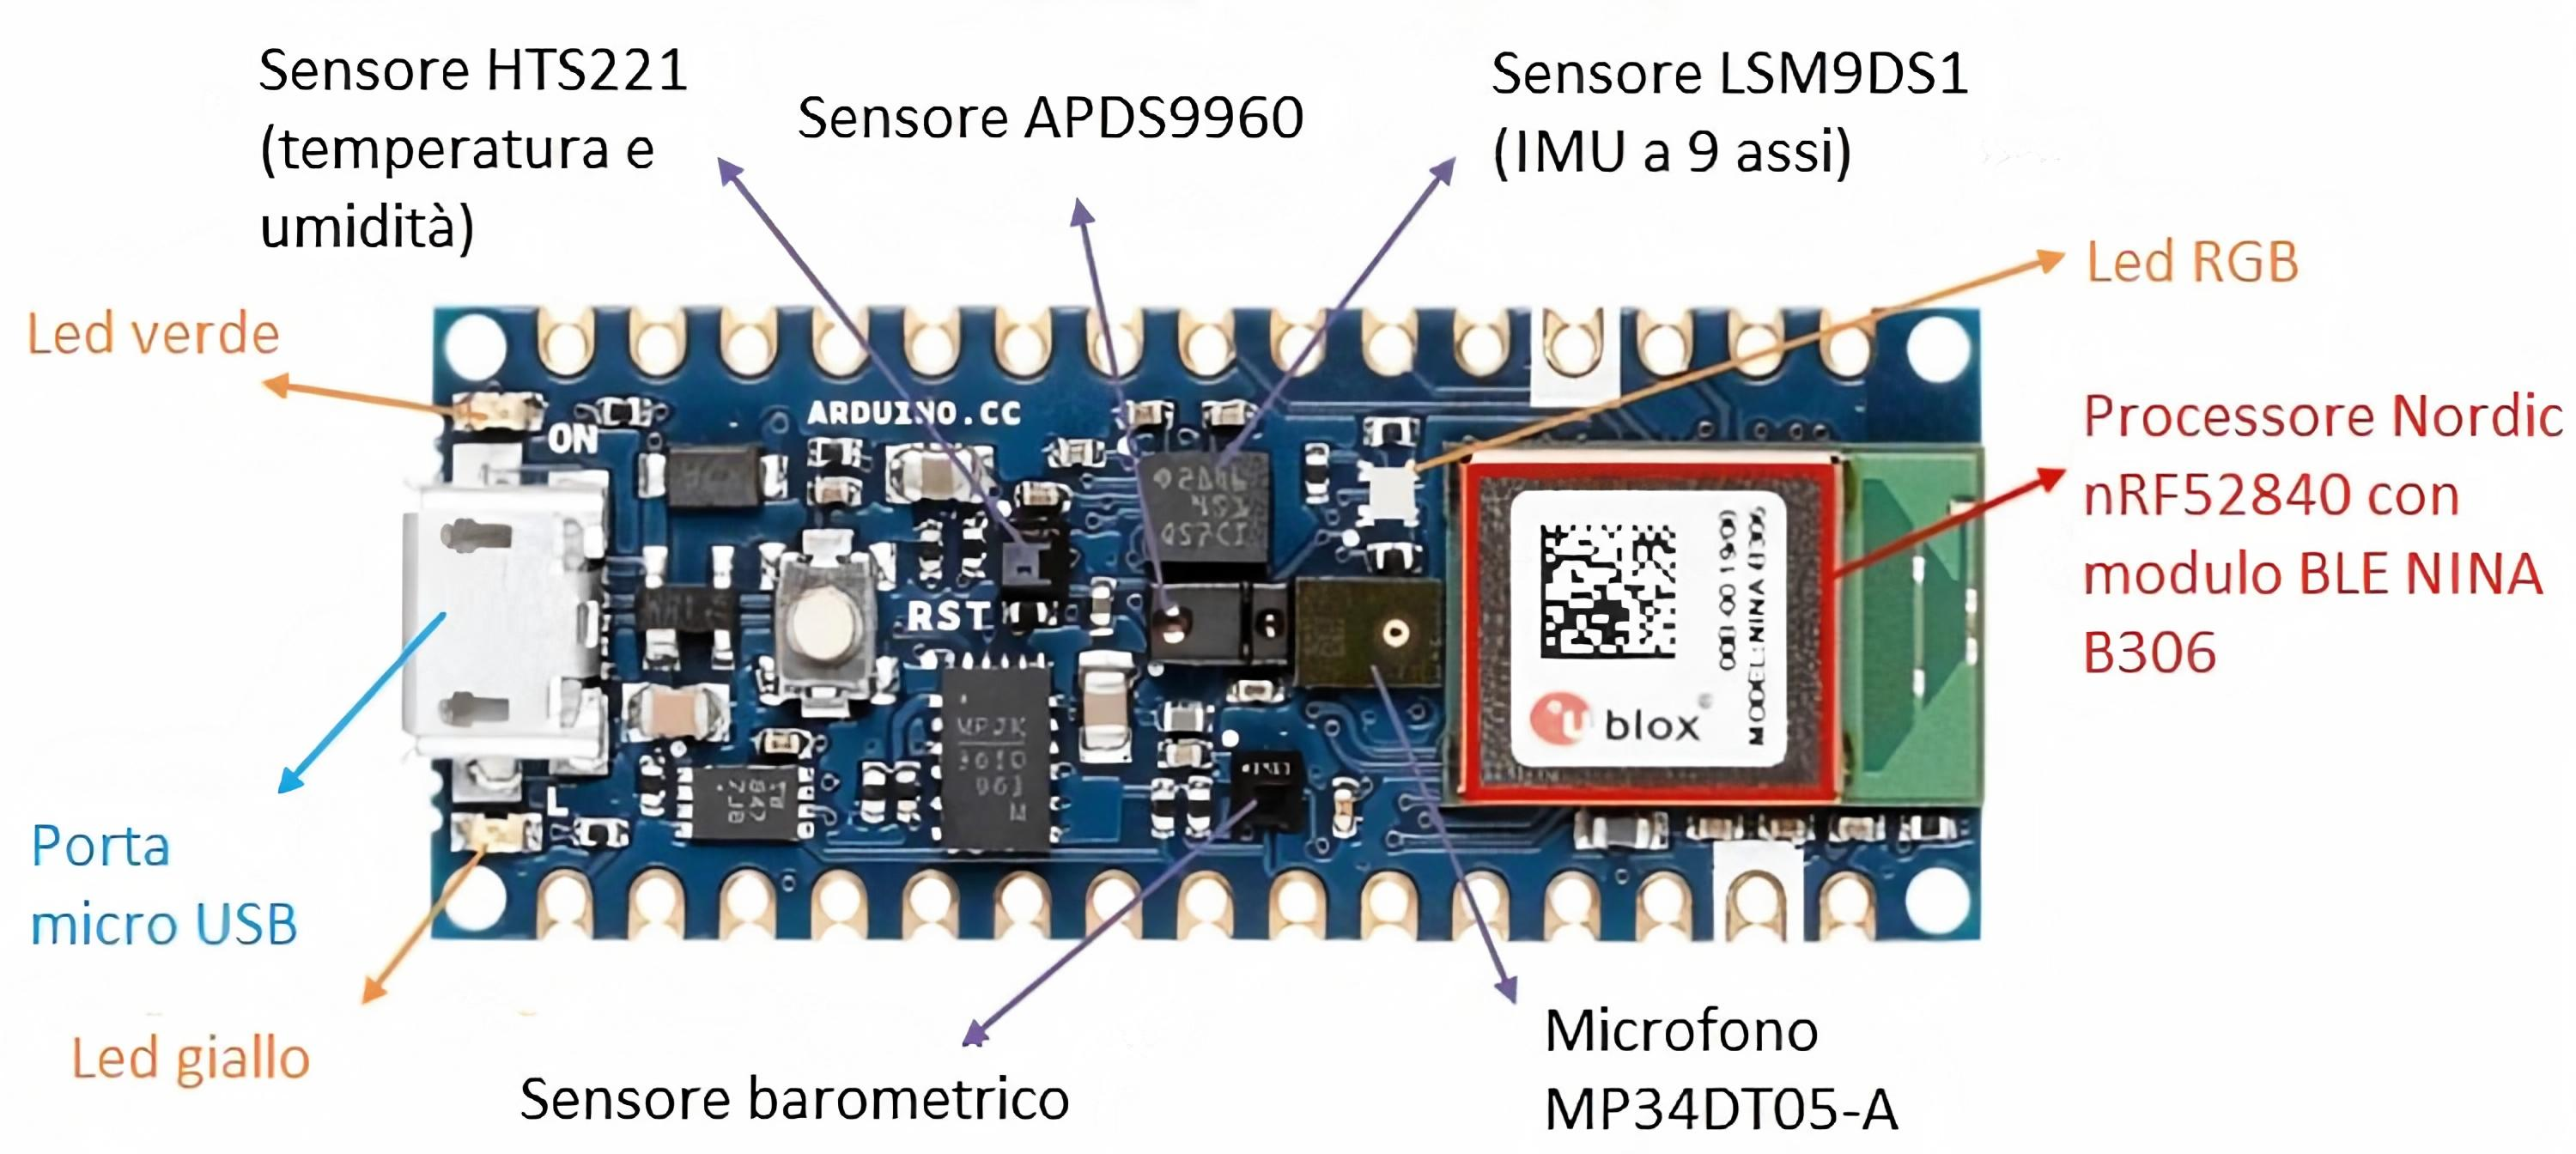
\includegraphics[width=\textwidth]{figures/Arduino_with_Sensors_4x.jpg}
    \caption{Scheda Arduino Nano 33 BLE - Nome e Posizione dei Componenti}
\end{figure}



\Attenzione{L'Arduino lavora a 3.3 V, di conseguenza accetta solamente voltaggi pari od inferiori a\\
\textbf{3.3 V}: se collegata a tensioni di valori superiori, la scheda potrebbe danneggiarsi}

\subsection{Specifiche Fondamentali della Scheda}
Di seguito ho riportato le informazioni ottenute\comment{prese}\comment{mostrate sulla} dalla pagina ufficiale sul sito Arduino, relative alla scheda di sviluppo: "Nano 33 BLE Sense"[\riferimento{100-chapter}{4}].\\
\begin{center} \begin{tabularx}{12,3cm}{|l l|}
\hline
    MICROCONTROLLER & nRF52840\\
    \hline
    OPERATING VOLTAGE & 3.3V\\
    INPUT VOLTAGE & 4.5V - 21V\\
    \hline
    DC CURRENT PER I/O PIN & 15 mA\\
    \hline
    CLOCK SPEED & 64MHz\\
    CPU\citCPU{} FLASH MEMORY & 1MB (nRF52840)\\
    SRAM\citSRAM{} & 256KB (nRF52840)\\
    EEPROM\citEEPROM{} & none\\
    \hline
    DIGITAL INPUT / OUTPUT PINS & 14\\
    PWM\citPWM{} PINS & all digital pins\\
    \hline
    UART\citUART{} & 1\\
    SPI\citSPI{} & 1\\
    I2C\citItwoC{} & 1\\
    \hline
    ANALOG INPUT PINS & 8 (ADC 12 bit 200 ksamples)\\
    ANALOG OUTPUT PINS & Only through PWM (no DAC)\\
    EXTERNAL INTERRUPTS & all digital pins\\
    \hline
    LED\_BUILTIN & 13\\
    \hline
    USB	Native in the & nRF52840 Processor\\
    \hline
\end{tabularx} \end{center}

\newpage{}


\section{Effetto Hall}\label{sezione 1-2}
L'effetto Hall è un fenomeno legato al passaggio di una corrente \textit{I} attraverso un conduttore, in una zona in cui è presente un campo magnetico, tramite questo fenomeno è possibile determinare due importanti caratteristiche del conduttore in questione: il segno dei portatori di carica e la loro densità [\riferimento{100-chapter}{5}].\\
Prende il nome dal fisico statunitense Edwin Hall, colui che ha scoperto questo effetto nel 1879 [\riferimento{100-chapter}{6}].\\
Indichiamo con \vettore{I} e \vettore{J} i due vettori che descrivono la corrente e la densità di corrente, rispettivamente, il cui verso è definito come: il verso in cui scorrerebbe la corrente, se i portatori di carica fossero positivi [\riferimento{100-chapter}{5}].\\
Rispetto alla velocità \vettore{v} dei portatori di carica, se questi ultimi sono portatori di carica positivi, allora \vettore{v} e \vettore{J} saranno paralleli; se invece i portatori di carica sono negativi i due vettori saranno antiparalleli [\riferimento{100-chapter}{5}].\\[7mm]

\label{IMAGE - Lastra di Metallo Sottoposta a corrente}
\begin{figure}[H]
    \centering
    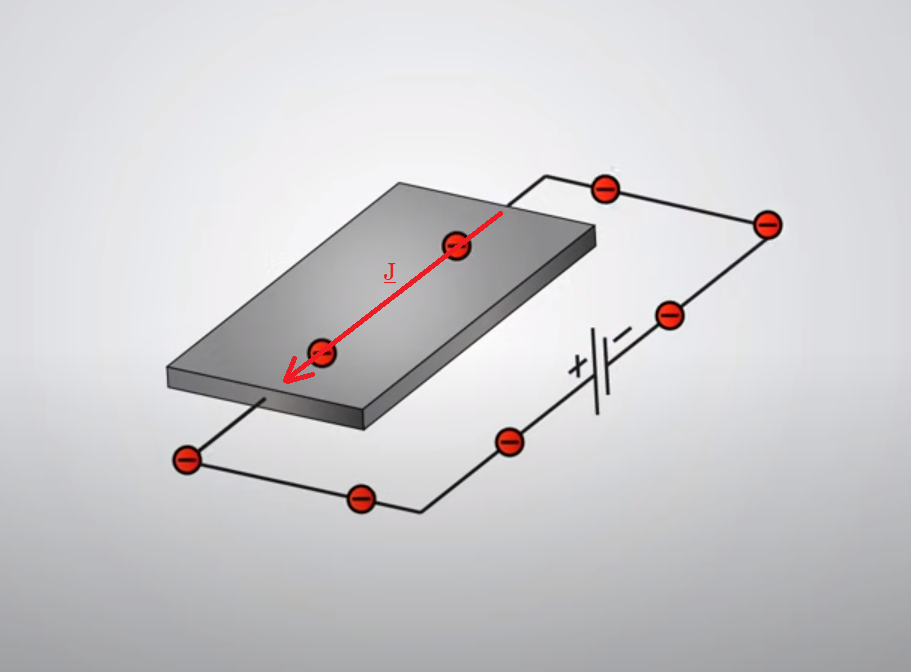
\includegraphics[width=\textwidth]{figures/Lastra di Metallo Sottoposta a corrente - Copia.PNG}
    \caption{Scorrimento di una corrente elettrica in una lastra di metallo}
\end{figure}

Supponiamo di avere un conduttore largo e sottile di superficie $S$, spessore $d$, \comment{e lo sottoponiamo} sottoposto ad un passaggio di corrente \vettore{I}, a cui corrisponde densità di corrente \vettore{J}, come illustrato in \riferimento{IMAGE - Lastra di Metallo Sottoposta a corrente}{Figura 1.2}.



Adesso si ipotizzi che la lastra di metallo sia soggetta ad un campo magnetico $\vec{B}$, come in \riferimento{IMAGE - Effetto della forza di Lorentz}{Figura 1.3}: tale campo modificherà il normale percorso della corrente, imponendogli una forza, in funzione del campo magnetico, detta "Forza di Lorentz".\\

\label{IMAGE - Effetto della forza di Lorentz}
\begin{figure}[H]
    \centering
    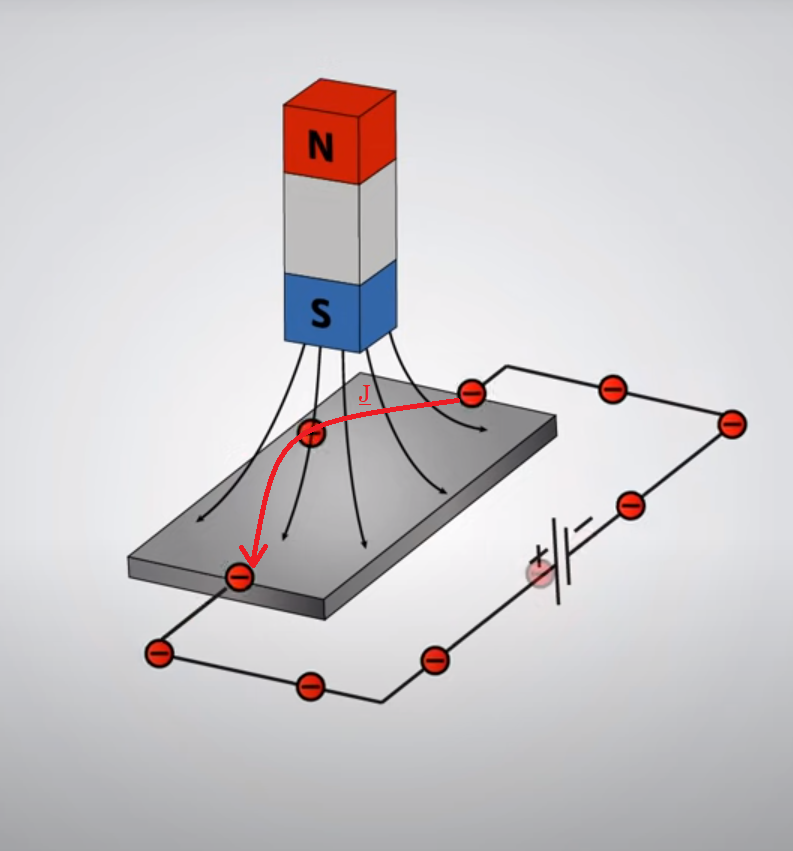
\includegraphics[width=145mm]{figures/Effetto_Hall_0 - Copia.PNG}
    \caption{Effetto della forza di Lorentz}
\end{figure}

Quindi, su ciascun portatore la forza impressa è:
\begin{equation} \label{eqn-1.1}
	\vec{F} = q\vec{v} \times{} \vec{B}
\end{equation}



In definitiva, a prescindere dal segno dei portatori di carica, ossia a prescindere
dal verso effettivo della corrente, l'azione del campo magnetico è sempre quella di
spingere trasversalmente (rispetto alla direzione della corrente) i portatori di carica,
addensandoli su un bordo del conduttore, come rappresentato in \riferimento{IMAGE - Misurazione dell'effetto Hall}{Figura 1.4}, portando così ad avere una differenza di potenziale $\Delta{}\varphi{}$ tra i bordi opposti del conduttore, che può essere misurata.\\
Basta allora stabilire il segno di questa differenza di potenziale per stabilire il segno dei portatori di carica.\\
La presenza di questa differenza di potenziale trasversale nei conduttori percorsi da corrente e soggetti ad un campo magnetico ad essa ortogonale, prende appunto il nome di "effetto Hall".[\riferimento{100-chapter}{5}].\\

\label{IMAGE - Misurazione dell'effetto Hall}
\begin{figure}[H]
    \centering
    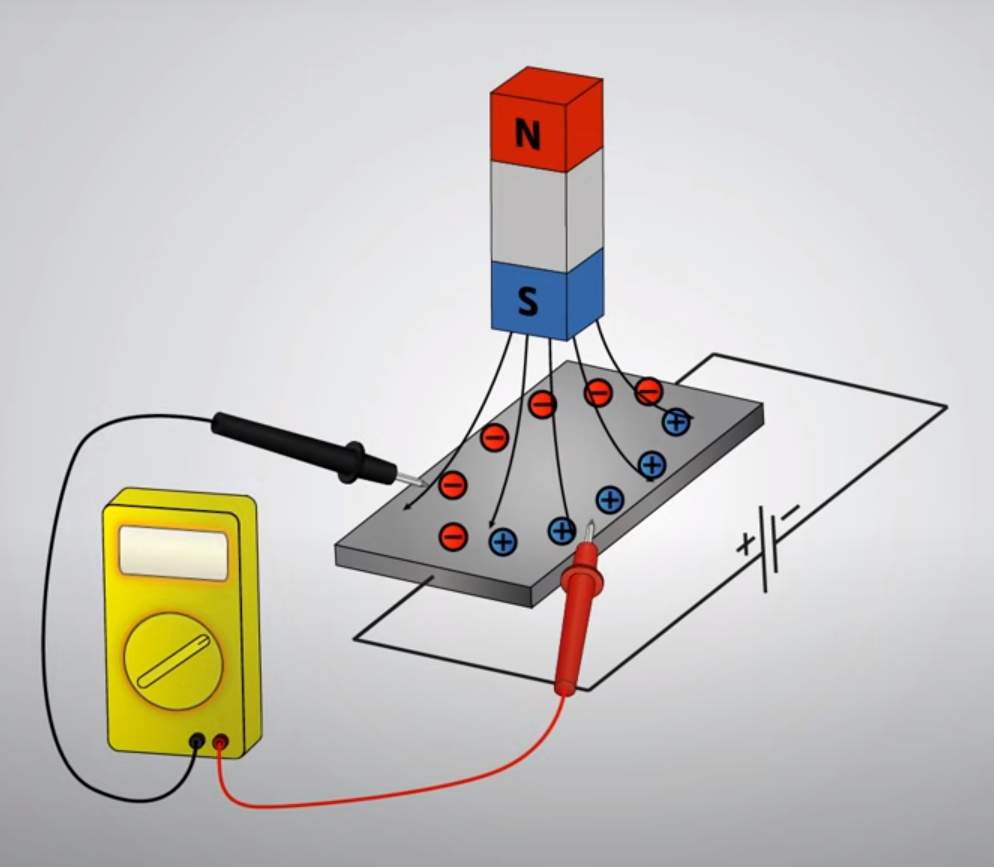
\includegraphics[width=\textwidth]{figures/Hall_effect_2.PNG}
    \caption{Misurazione dell'effetto Hall}
\end{figure}

\newpage{}

Il fatto che la forza di Lorentz faccia accumulare i portatori di carica su un bordo del conduttore, con conseguente creazione di una differenza di potenziale tra i due bordi opposti del conduttore, fa sì che si crei un campo elettrico \vettore{E_h} trasversale, diretto cioè ortogonalmente alla direzione della corrente. \\
Di conseguenza, quanta più corrente scorre, tanti più portatori vengono spinti dalla forza di Lorentz, e tanto maggiore sarà il valore di \vettore{E_h}; quindi se scorre più corrente, maggiore sarà la forza \vettore{F_h} che il campo elettrico trasversale esercita sugli stessi portatori [\riferimento{100-chapter}{5}].\\

\subsection{Differenza di potenziale data dall'effetto Hall}

Ricordiamo che comunque la forza elettrica \vettore{F_h} si oppone sempre alla forza magnetica, quindi, a prescindere dal segno dei portatori di carica, arriverà un momento in cui le due forze si equilibrano perfettamente,
cioè quando la forza di Lorentz risulta nulla:[\riferimento{100-chapter}{5}].

\begin{equation} \label{eqn-1.2}
	\vec{F} = q\vec{v} \times{} \vec{B} + q\vec{E_h} = 0
\end{equation}

Ricavando il valore del campo elettrico $\vec{E_h}$, all’equilibrio:
\begin{equation} \label{eqn-1.3}
	\vec{E_h} = -\vec{v} \times{} \vec{B}
\end{equation}

La velocità da considerare deve essere quella media dei portatori di carica, per
cui la relazione diventa:
\begin{equation} \label{eqn-1.4}
	\vec{E_h} = -\langle{}\vec{v}\rangle{} \times{} \vec{B}
\end{equation}

Indichiamo con N il numero totale di portatori di carica per unità di volume, possiamo quindi ricavare la densità di corrente:
\begin{equation} \label{eqn-1.5}
	\vec{J} = Nq\langle{}\vec{v}\rangle{}
\end{equation}

Da cui ricaviamo che:
\begin{equation} \label{eqn-1.6}
	\langle{}\vec{v}\rangle{} = \frac{\vec{J}}{Nq}
\end{equation}

Sostituendo nell’espressione del campo elettrico (1.4) , otteniamo:
\begin{equation} \label{eqn-1.7}
	\vec{E_h} = -\frac{1}{Nq} \cdot{} (\vec{J}\times{}\vec{B})
\end{equation}

Per definizione, la densità di corrente che scorre lungo il conduttore è data, in
modulo, dal rapporto tra la corrente $I$, e l’area $S$ del conduttore attraversata dalla
corrente stessa: considerando che abbiamo definito il conduttore con uno spessore $d$ e e larghezza $l$,\\ si deduce che: \comment{[\riferimento{100-chapter}{5}]}
\begin{equation} \label{eqn-1.9}
	S = d\cdot{}
\end{equation}
per cui: \\
\begin{equation} \label{eqn-1.9}
	J = \frac{I}{d\cdot{}}
\end{equation}

Sostituendo nella espressione del campo elettrico (1.7) e calcolando il modulo di tale campo, abbiamo:
\begin{equation} \label{eqn-1.8}
	\vec{E_h} = -\frac{J\cdot{}B}{Nq}sin\theta{} = -\frac{I\cdot{}B}{Nq\cdot{}d\cdot{}l}sin\theta{}
\end{equation}

Dove con $\theta{}$ viene indicato l’angolo formato dai vettori $\vec{J}$ e $\vec{B}$.\\
Se consideriamo $\theta{} = \pi{}/2$, ipotizzando che il campo \vettore{B} sia ortogonale alla direzione della corrente, avremo che il modulo del campo elettrico trasversale è:
\begin{equation} \label{eqn-1.9}
	\vec{E_h} = -\frac{I\cdot{}B}{Nq\cdot{}d\cdot{}l}sin\theta{} 
\end{equation}

Dal valore del campo all’equilibrio, si può risalire al valore della differenza di
potenziale \vettore{V_h} all’equilibrio:
\begin{equation} \label{eqn-1.10}
	\vec{V_h} = -\vec{E_h}\cdot{}l =  -\frac{I\cdot{}B}{Nq\cdot{}d}sin\theta{} 
\end{equation}

\myNOTE{
Si deduce che, a parità di forma del conduttore e a parità di campo magnetico, la\\
differenza di potenziale che si manifesta ai bordi del conduttore (una volta raggiunto\\
l’equilibrio) cresce proporzionalmente al crescere di $\vec{I}$, ed al diminuire del fattore $N\cdot{}q$,\\
che è appunto la densità spaziale di carica e che si può ricavare dalla relazione (1.11) [\riferimento{100-chapter}{5}].
}

\comment{ %Dont know if this figure is usefull or not
\label{}
\begin{figure}[H]
    \centering
    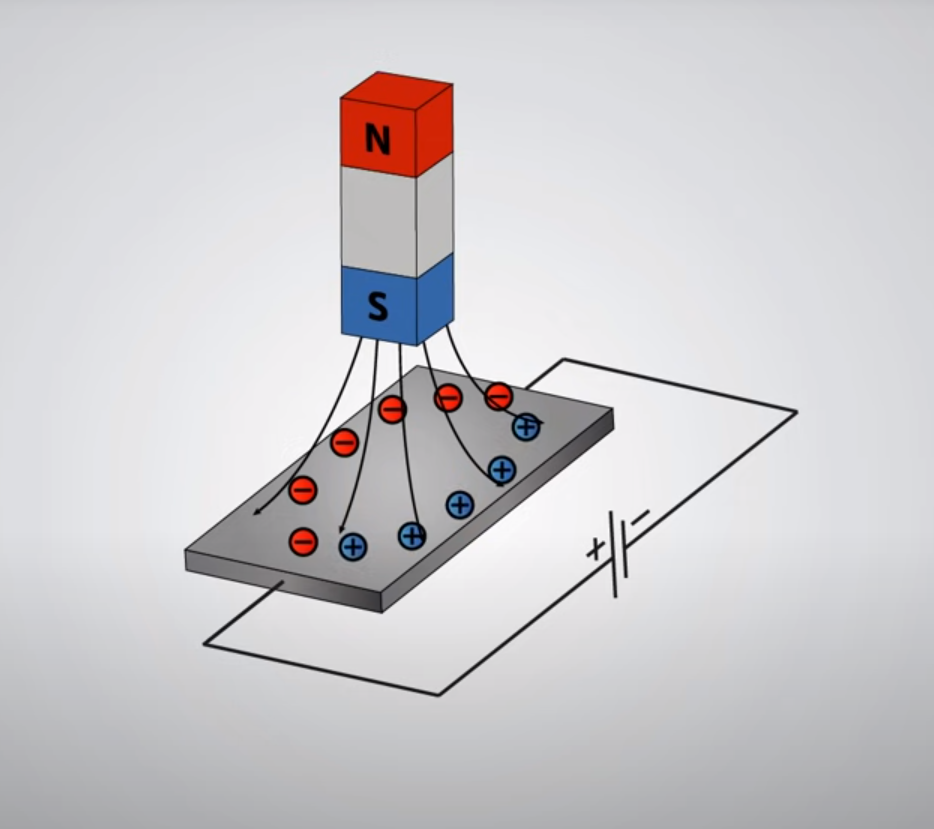
\includegraphics[width=\textwidth]{figures/Effetto Hall 1.PNG}
    \caption{}
\end{figure}
}

\newpage{}

\section{Sensori ad Effetto Hall}\label{sezione 1-3}
La famiglia A130 (A1301 e A1302) è composta da\comment{comprende} sensori \comment{a tempo continuo,}raziometrici lineari che sfruttano l'effetto Hall per fornire in uscita una tensione proporzionale al campo magnetico applicato.
\comment{Entrambi i dispositivi hanno una tensione in uscita a riposo,\comment{ovvero}\comment{in assenza di un campo magnetico} definita come la tensione in uscita in assenza di campo magnetico , pari al 50\% della tensione di alimentazione.}\\
Tutti i dispositivi appartenenti alla famiglia A130, in assenza di\comment{non soggetti ad} un campo magnetico significativo, presentano in uscita una tensione così detta "a riposo", pari al\comment{definita come il } 50\% della tensione di alimentazione.
Lo specifico sensore che andremo ad utilizzare (A1301) ha una sensibilità tipica pari ad $1.3$ $\mathrm{\frac{mV}{G}}$ [\riferimento{100-chapter}{7}].\\

Il circuito integrato ad effetto Hall, presente in ogni sensore, include un sensore di Hall, un amplificatore lineare ed una struttura CMOS di Classe A come stadio di uscita, lo schema a blocchi del sensore è riportato in \riferimento{IMAGE - Functional Block Diagram}{Figura 1.5}.\\
Integrare il sensore di Hall e l’amplificatore su un unico chip minimizza molti dei problemi normalmente associati a segnali analogici a basso livello di tensione [\riferimento{100-chapter}{7}].\\
Un’alta precisione nei livelli di uscita, viene inoltre ottenuta grazie ad una regolazione dell’offset, effettuata come ultimo passo del processo di produzione\comment{effettuata come ultimo passaggio, durante il processo di produzione} [\riferimento{100-chapter}{7}].\\

\label{IMAGE - Functional Block Diagram}
\begin{figure}[H]
    \centering
    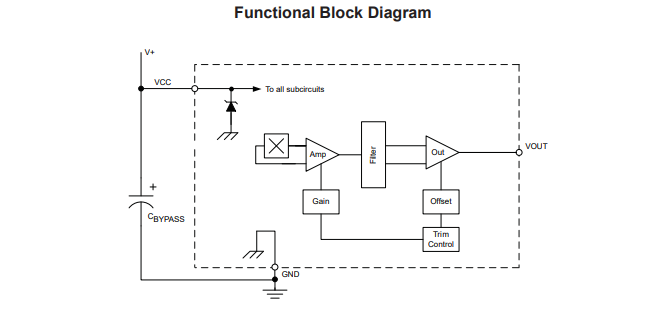
\includegraphics[width=\textwidth]{figures/Functional Block Diagram.PNG}
    \caption{Sensore ad effetto Hall A1302 - Functional Block Diagram}
\end{figure}

\label{IMAGE - Datasheet}
\begin{figure}[H]
    \centering
    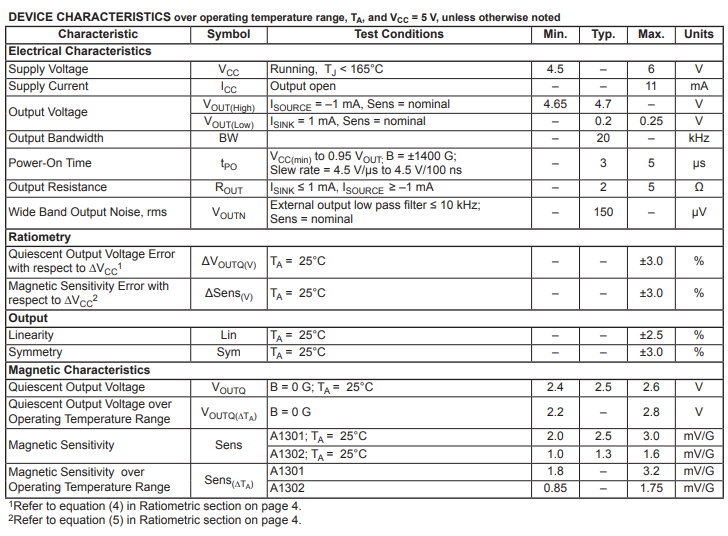
\includegraphics[width=135mm]{figures/Datasheet.PNG}
    \caption{Sensore ad effetto Hall A1302 - Datasheet}
\end{figure}

\label{IMAGE - Pin Out Drawings}
\begin{figure}[H]
    \centering
    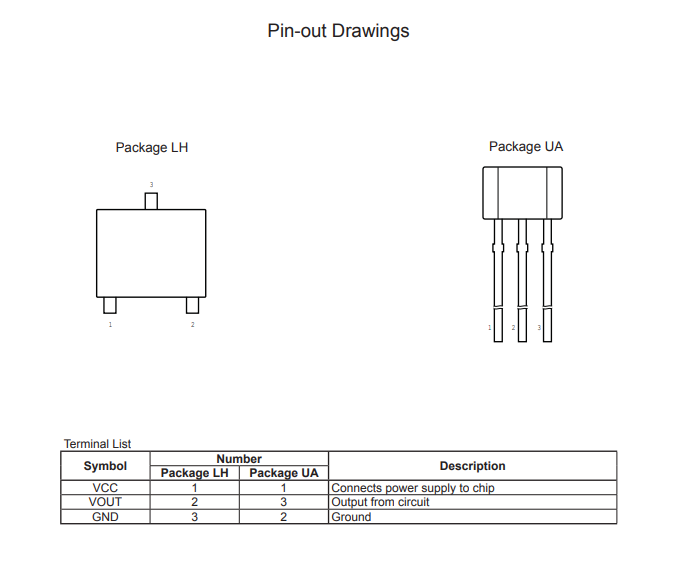
\includegraphics[width=125mm]{figures/Pin Out Drawings.PNG}
    \caption{Sensore ad effetto Hall A1302 - Pin Out Drawings}
\end{figure}

Come possiamo vedere in \riferimento{IMAGE - Functional Block Diagram}{Figura 1.7} sono disponibili due tipi di package per lo stesso dispositivo: LH, a 3-pin SOT23W specifico per il montaggio superficiale, ed il pacchetto UA, a 3-pin ultramini SIP per il montaggio a foro passante.\\
Entrambi i pacchatti sono senza piombo (Pb) ed i leadframes sono completamente placcati in stagno opaco\comment{ matte tin plated leadframes}.

\label{IMAGE - vs. Suplly Voltage}
\begin{figure}[H]
    \centering
    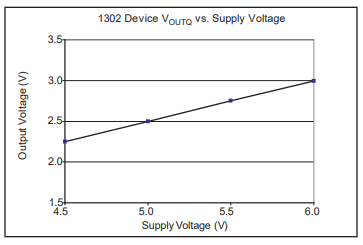
\includegraphics[width=75mm]{figures/Device Voutq vs. Supply Voltage.PNG}
    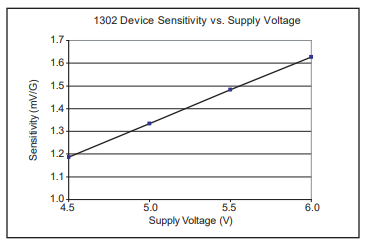
\includegraphics[width=75mm]{figures/Device Sensitivity vs. Supply Voltage.PNG}
    \caption{Sensore ad effetto Hall A1302 - Vout at Quiescent State and Sensitity vs. Supply Voltage}
\end{figure}

\textbf{Tensione in uscita a riposo}:\\
Quando il sensore si trova in uno stato di riposo (nessun campo magnetico significativo: \vettore{B}=0 T), in uscita $V_{outq}$ assume un valore pari a metà della tensione di alimentazione $V_{cc}$.
Data la temperatura ambiente $T_A$ ed il range della tensione di alimentazione $V_{cc}$, è possibile calcolare\comment{trovare} una tolleranza sulla tensione a riposo, $\Delta{}V_{outq}$, in funzione di $\Delta{}V_{cc}$ e $\Delta{}T_A$, viene definita come:
\begin{equation} \label{eqn-1.10}
	\Delta{}V_{outq}(\Delta{}T_A) = \frac{\Delta{}V_{outq}(T_A) - \Delta{}V_{outq}(25^{\circ{}})}{Sens(25^{\circ{}})}
\end{equation}
dove "$Sens$" si misura in $\mathrm{\frac{mV}{G}}$ ed \comment{il risultato assume il significato di}indica la sensitività del dispositivo\comment{il risultato finale espresso in Gauss (G), indica l'accuratezza del sensore, applicabile su tutto il range di temperatura}.\\

\textbf{Razionometrico}:\\
Il sensore A1301 è caratterizzato da un'uscita razionometrica, ciò vuol dire sia la $V_{outq}$, che la sensibilità magnetica, $Sens$, sono proporzionali alla tensione di alimentazione $V_{cc}$.
La percentuale di cambiamento (\%) della tensione in uscita a riposo è definita come:
\begin{equation} \label{eqn-1.10}
	\Delta{}V_{outq}(\Delta{}V) = \frac{V_{outq}(V_{cc}) / V_{outq}(5V)}{V_{cc} / 5V} \times{} 100\%
\end{equation}
Mentre il \textit{ratiometric change} (\%) per la Sensitività è definito come:
\begin{equation} \label{eqn-1.10}
	\Delta{}Sens(\Delta{}V) = \frac{Sens(V_{cc}) / Sens(5V)}{V_{cc} / 5V} \times{} 100\%
\end{equation}

\newpage{}

\textbf{Sensitività}:\\ 
La presenza di un campo magnetico a polarità positiva ($+{B}$), perpendicolare alla parte frontale del dispositivo, aumenta la tensione di uscita $V_{out}$, in proporzione al campo magnetico applicato, da $V_{outq}$ fino ad un massimo pari a $V_{cc}$.\\
Al contrario se si ha di fronte \comment{alla polarità negativa di campo magnetico}la polarità negativa di un campo magnetico ($-{B}$), nella stessa orientazione, ridurrà proporzionalmente $V_{out}$ da  $V_{outq}$ fino ad un minimo pari a 0 V.\\
La proporzionalità di queste variazioni è definita come la sensibilità magnetica del dispositivo:
\begin{equation} \label{eqn-1.10}
	Sens = \frac{V_{out}(-B) + V_{out}(+B)}{2B}
\end{equation}
La stabilità della sensibilità magnetica del dispositivo è una funzione della temperatura ambiente, $\Delta{}Sens(\Delta{}T_A)$ in percentuale (\%) è definita come:
\begin{equation} \label{eqn-1.10}
	\Delta{}Sens(\Delta{}T_A) = \frac{Sens(T_A) - Sens(25^{\circ{}})}{Sens(25^{\circ{}})} \times{} 100\%
\end{equation}

\textbf{Simmetria e Linearità}:\\
Lo stadio di uscita montato sul chip è costruito per fornire un'uscita lineare, se fornita una tensione di alimentazione pari a 5 V.\\
Anche se l'applicazione di forti campi magnetici non danneggiano il dispositivo, forzano però l'uscita in una zona di non-linearità.\\
La linearità in percentuale è misurata come segue:
\begin{equation} \label{eqn-1.10}
	Lin+ = \frac{V_{out}(+B) - V_{outq}}{2(V_{out}(+B\frac{1}{2}) - V_{outq})} \times{} 100\%
\end{equation}
\begin{equation} \label{eqn-1.10}
	Lin- = \frac{V_{out}(-B) - V_{outq}}{2(V_{out}(-B\frac{1}{2}) - V_{outq})} \times{} 100\%
\end{equation}
e la simmetria di uscita come:
\begin{equation} \label{eqn-1.10}
	Sym = \frac{V_{out}(+B) - V_{outq}}{V_{outq}) - V_{out}(-B)} \times{} 100\%\\[4mm]
\end{equation}

Riportate in \comment{questa scheda}questo paragrafo i grafici relativi alla tensione a riposo, ed alla sensibilità del dispositivo in rispetto alla tensione di alimentazione, in \riferimento{IMAGE - vs. Suplly Voltage}{Figura 1.8}, che saranno poi utili nell'utilizzo pratico del sensore[\riferimento{100-chapter}{7}].

\newpage{}

\section{Edge Impulse}\label{sezione 1-4}
Edge Impulse[\riferimento{100-chapter}{1}], ovvero TinyML come servizio, consente l'utilizzo dell'apprendimento automatico a tutti gli sviluppatori con un SDK (Software Development Kit) per dispositivi open source, sfruttando principalmente due librerie: "TensorFlow" per l'addestramento della rete neurale, e "TensorFlow Lite" per l'utilizzo su sistemi embedded.\\

Dalla pagina web è possibile: raccogliere dati da vari sensori, elaborare segnali in tempo reale, effettuare test \comment{e distribuire}su qualsiasi dispositivo\comment{supportato} [\riferimento{100-chapter}{8}].\\
%Gli SDK open source offerti da Edge Impulse consentono di raccogliere dati o distribuire codice su qualsiasi dispositivo [\riferimento{100-chapter}{8}].\\
In particolare viene offerta la possibilità di ottenere il modello di machine learning "TensorFlow Lite", dopo averlo addestrato, sia in un file di formato ".tflite", \comment{dopo averlo\comment{una volta} addestrato}come libreria Arduino (che vedremo in particolare nel prossimo Capitolo), \comment{ovviamente modificabile}oppure come libreria C++, Cube.MX CMSIS-PACK, WebAssembly o TensorRT.\\

Viene inoltre offerta la possibilità di inviare raccolte di dati tramite file con estensione:
\begin{itemize}[noitemsep]
    \item{".CBOR"}
    \item{".JSON"}
    \item{".CSV"}
    \item{".WAV" (per file audio)}
    \item{".JPG" (per immagini)}
    \item{".PNG" (per immagini)}\\
\end{itemize}

Edge Impulse è una piattaforma di sviluppo, gratuita per i singoli sviluppatori, che gli utenti possono contribuire ed estendere, aggiungendo e modificando algoritmi di machine learning, o implementando supporti per nuovi dispositivi. Il software del dispositivo, inclusi SDK, client, e codice generato, viene fornito come open source con una licenza Apache 2.0 [\riferimento{100-chapter}{8}].\\


\clearpage\null\thispagestyle{empty}

\chapter{Implementazione}


% DICHIARAZIONE myFOOTNOTES
\newcommand{\citPORVA}{\nota{PORVA: Inertial Measurement Unit}{}}

%%%%% Capitolo 1 %%%%%

\label{02-chapter}
%\usepackage{wrapfig}
\begin{wrapfigure}{l}{90mm}
  \begin{center}
    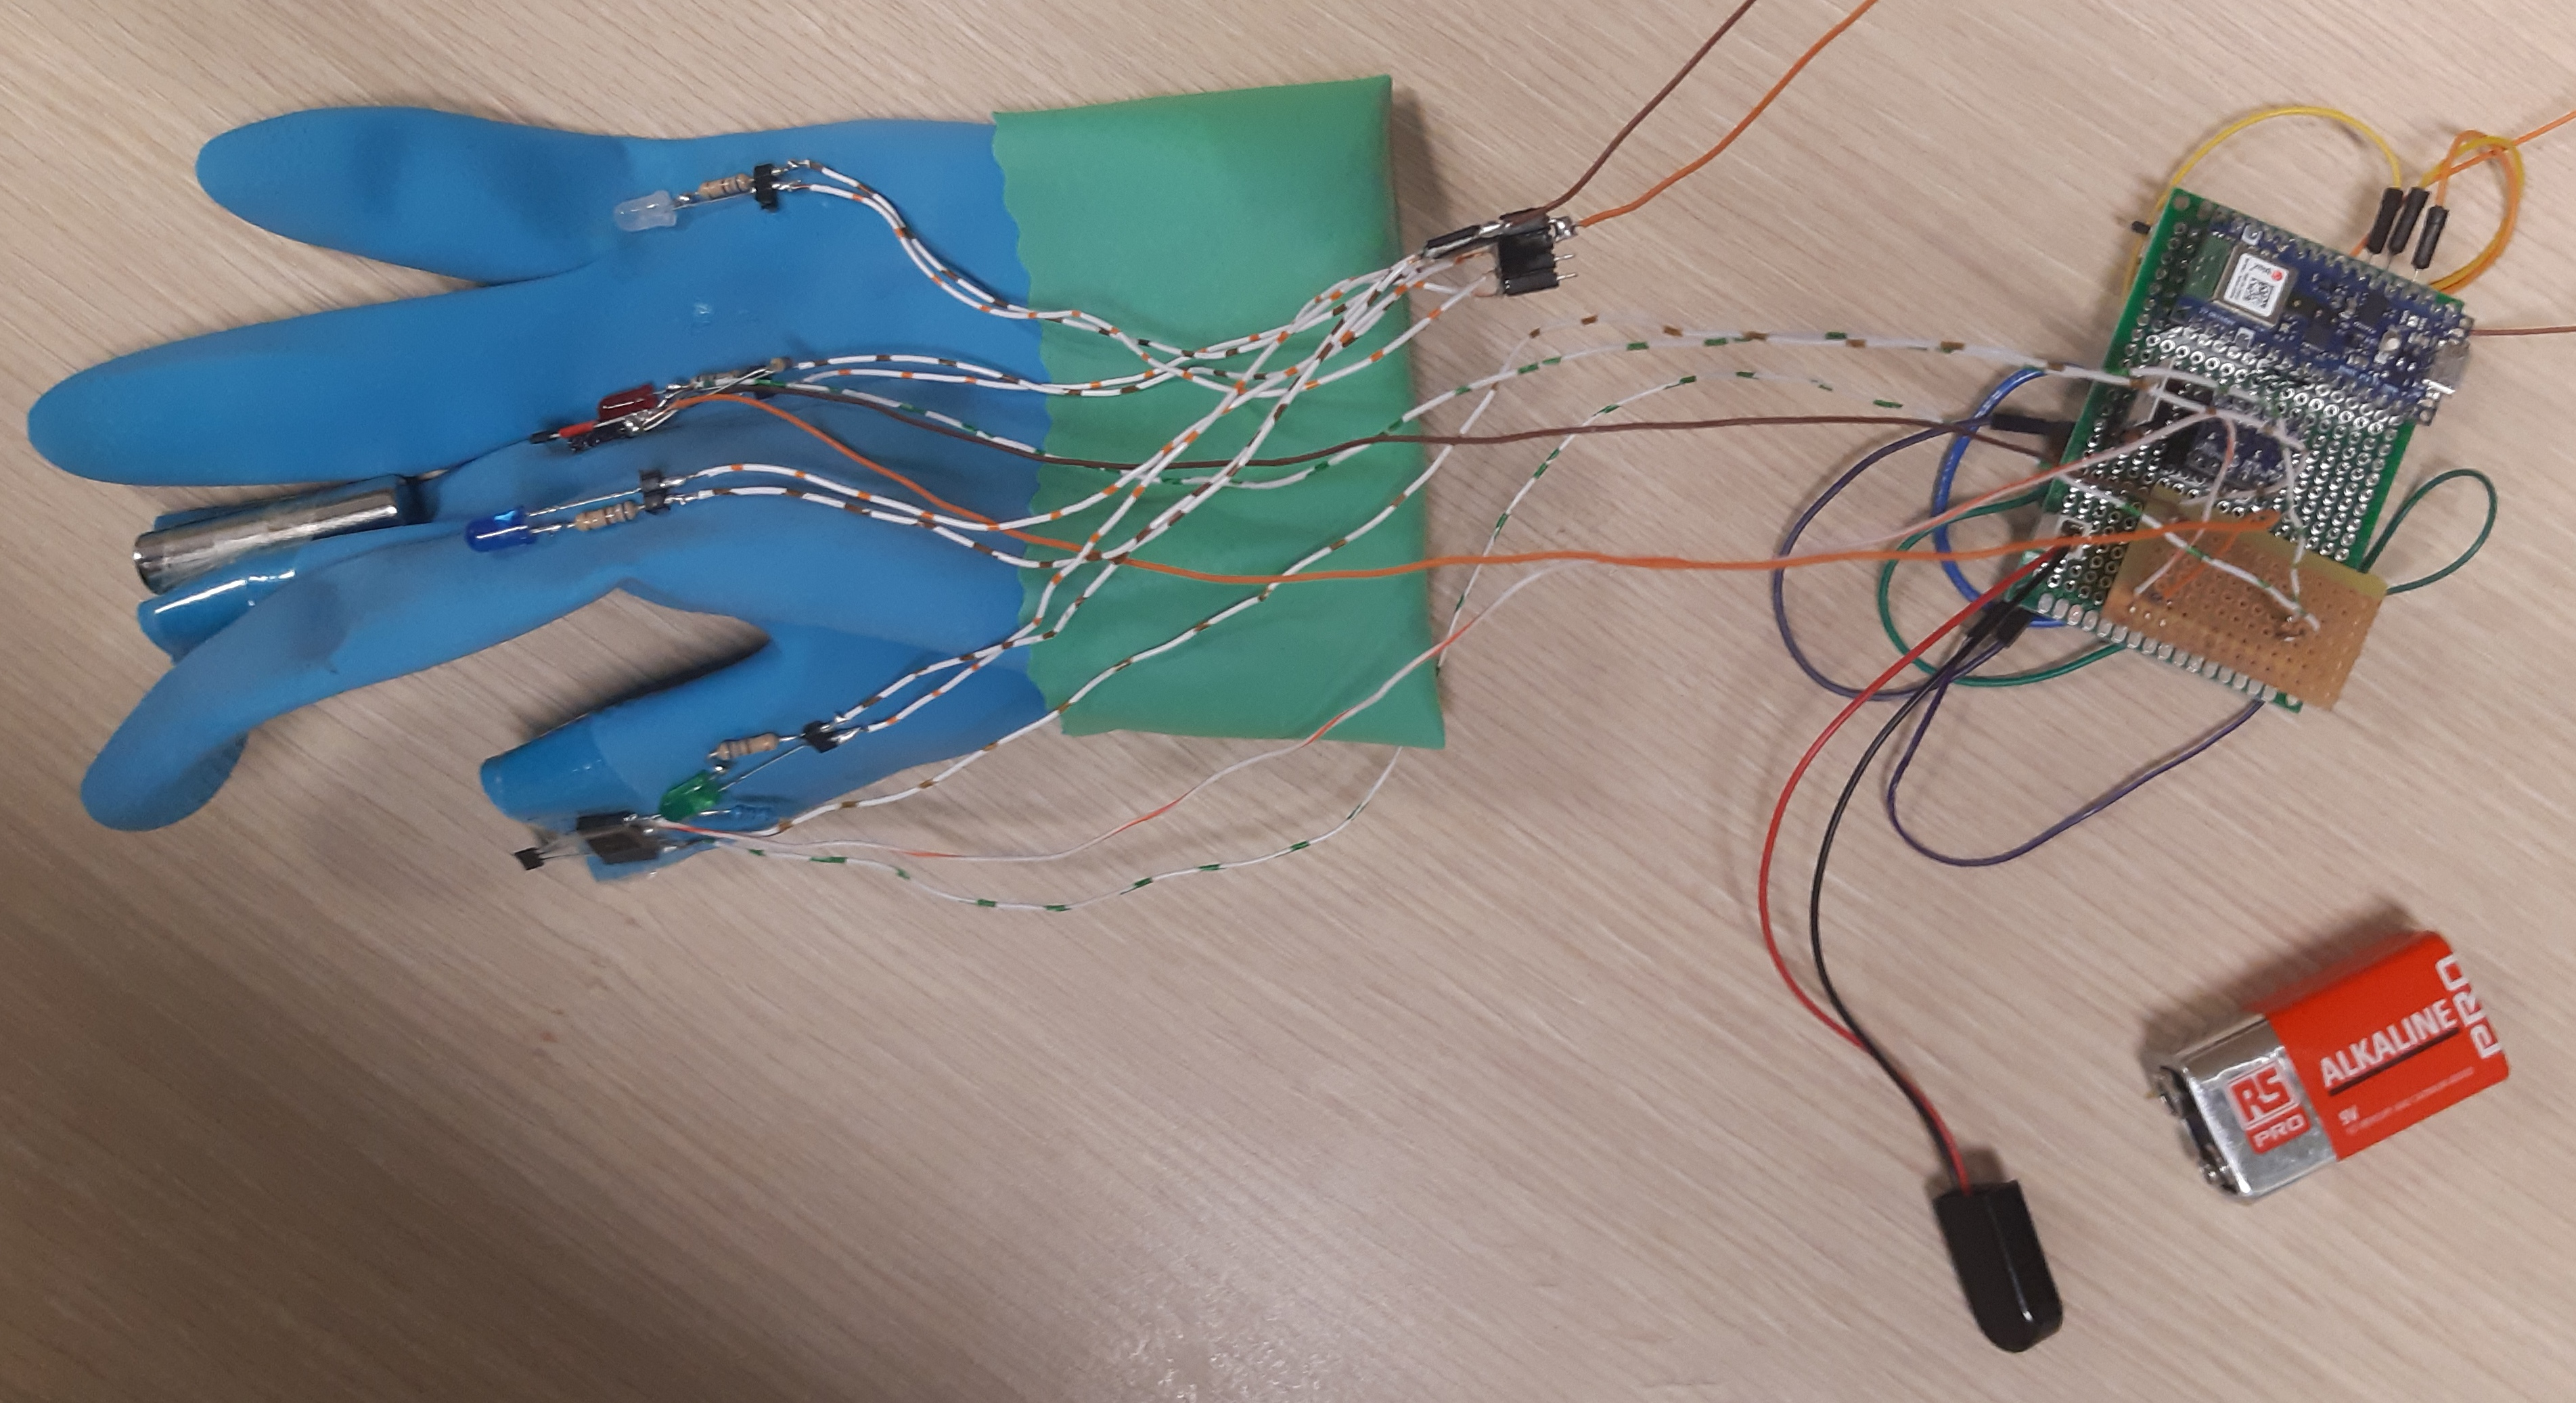
\includegraphics[width=0.48\textwidth]{figures/Guanto_Finale (1).jpg}
  \end{center}
    \caption{Immagine Finale del Guanto per il Riconoscimento di uno Schiocco di Dita}
%\end{wrapfigure}
\end{wrapfigure}

Utilizzando due sensori di Hall, posizionati su un guanto di gomma, uno sul retro del pollice e l'altro sulla nocca del dito medio, una calamita attaccata al retro del medio, e l'Arduino Nano 33 BLE Sense sul quale è caricato lo sketch con il modello di machine learning, sono stato in grado di rivelare quando vengono fatte schioccare le dita,\comment{e se la rete neurale ha una confidenza che reputo sufficiente} e quando accade \comment{attivo}4 led incollati sul guanto si accendono.\\

Il flusso di lavoro\comment{workflow} che ho adottato è il seguente:
\par

\begin{itemize}
    \item {Raccolta dei dati dai sensori tramite sketch Arduino, che dovranno poi essere scritti sulla porta seriale, sempre dallo stesso sketch.}
    \item {Collezione dei dati scritti sul seriale, e salvataggio degli stessi su fogli con estensione ".csv", tramite script python.}
    \item {Inoltro dei file ".csv" appena creati sulla piattaforma Edge Impulse, con seguente creazione ed allenamento della rete neurale, che verrà poi inserita in una libreria Arduino per il dislocamento sulla scheda Nano.}
    \item {Infine, creazione di un nuovo sketch Arduino per l'utilizzo della libreria fornita da Edge.}\\
\end{itemize}

\newpage{}



\section{Raccolta Dati tramite Sketch Arduino} \label{sezione 2-1}
Per prima cosa ho creato un semplice prototipo su breadboard in cui ho collegato una scheda Arduino UNO come mostrato in \riferimento{IMAGE - GDA ARDUINO UNO}{Figura 2.2}.
Ho usato questa scheda in una prima prova, per la possibilità dell'Arduino UNO di inviare e ricevere segnali a 5 V, visto che i sensori devono essere alimentati a 5 V, ed i valori in uscita dal sensore hanno range tra\\ 0 V - 5 V, valori che normalmente \textbf{non} possono essere accettati, come scritto in precedenza, dall'Arduino Nano.
Questo problema è facilmente risolvibile con convertitori di tensione generici per \\5 V$\rightarrow{}$3.3 V, convertitori che sono stati infatti adottati in seguito.\\

\label{IMAGE - GDA ARDUINO UNO}
\begin{figure}[H]
    \centering
    \caption{Esempio di hardware per la lettura dei sensori Hall}
    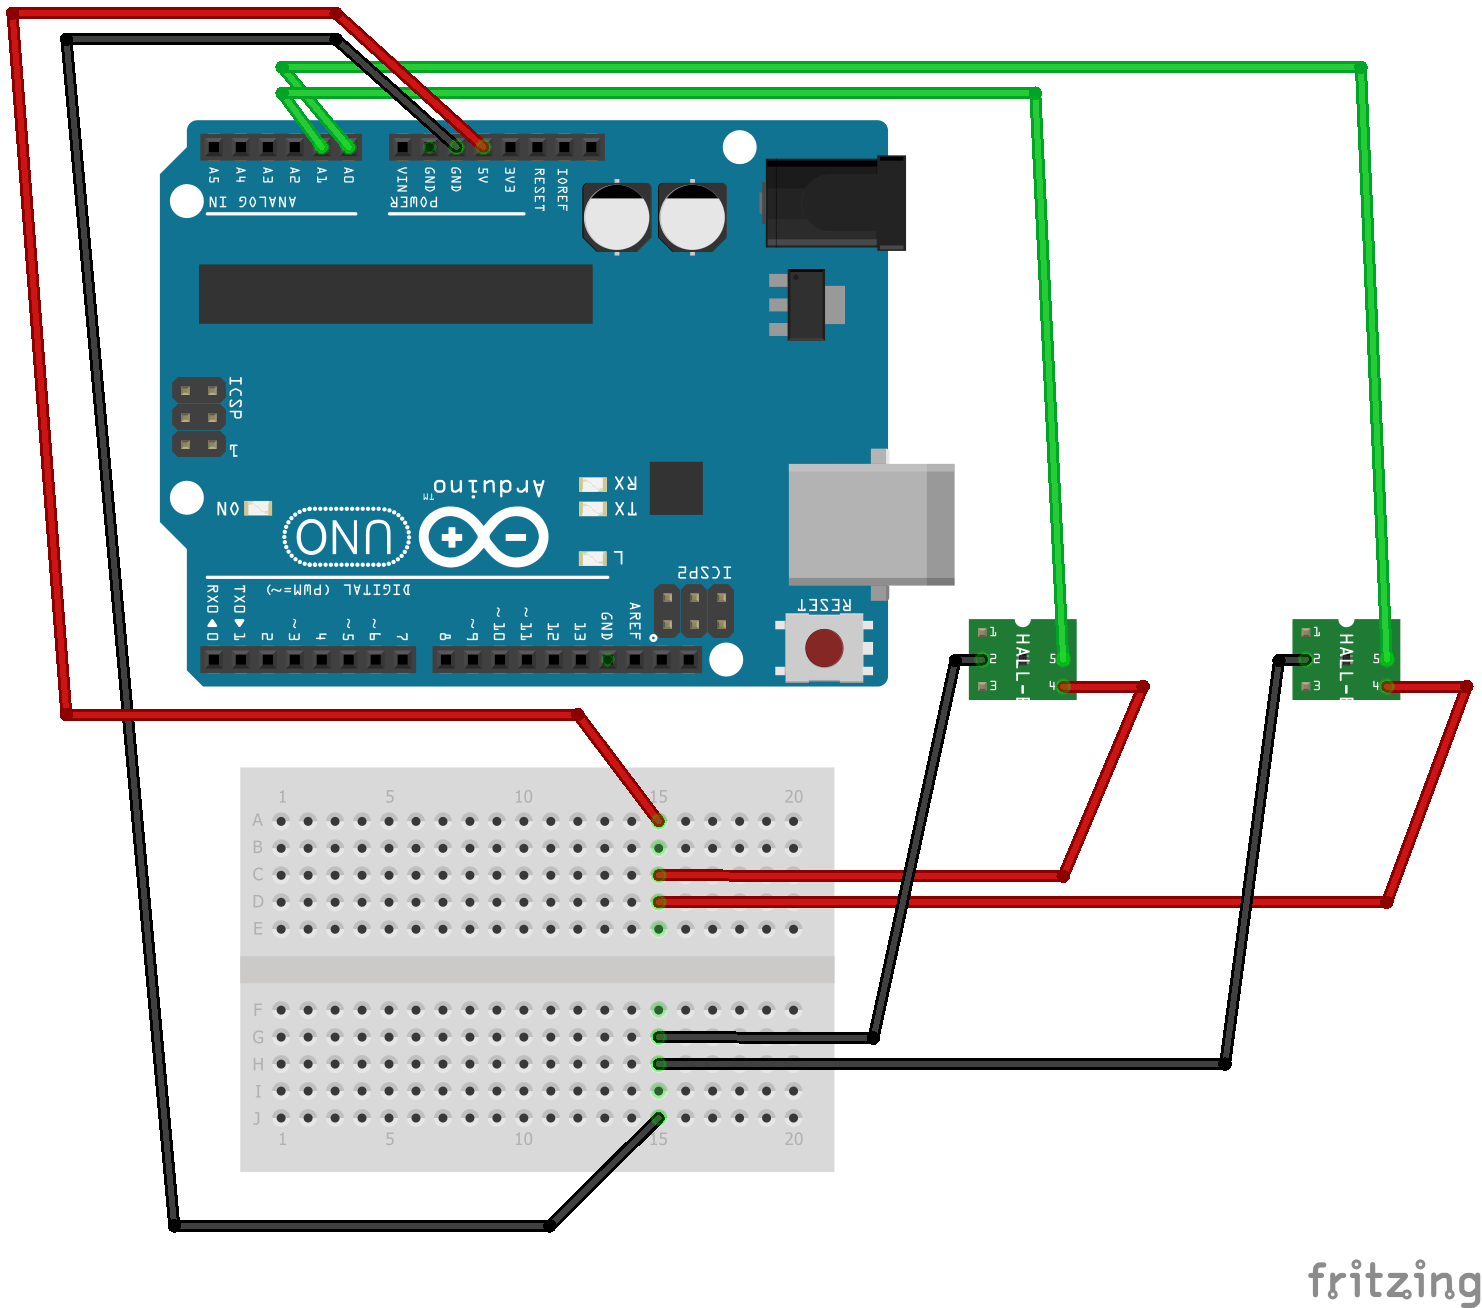
\includegraphics[width=\textwidth]{figures/Fritzing - GDA_from_Hall_Sensors_I.png}
\end{figure}

\newpage{}

Una volta visto come raccogliere dati, e scelto un magnete tra quelli disponibili in laboratorio, che dia una variazione consistente se mosso vicino ai sensori, ho portato il progetto sull'Arduino Nano, tramite vari shifter di tensione, come accenato prima, ed alimentando il tutto a batteria (9 V). Lo schema del progetto è mostrato nella \riferimento{IMAGE - GDA ARDUINO NANO}{Figura 2.3}:
\label{IMAGE - GDA ARDUINO NANO}
\begin{figure}[H]
    \centering
    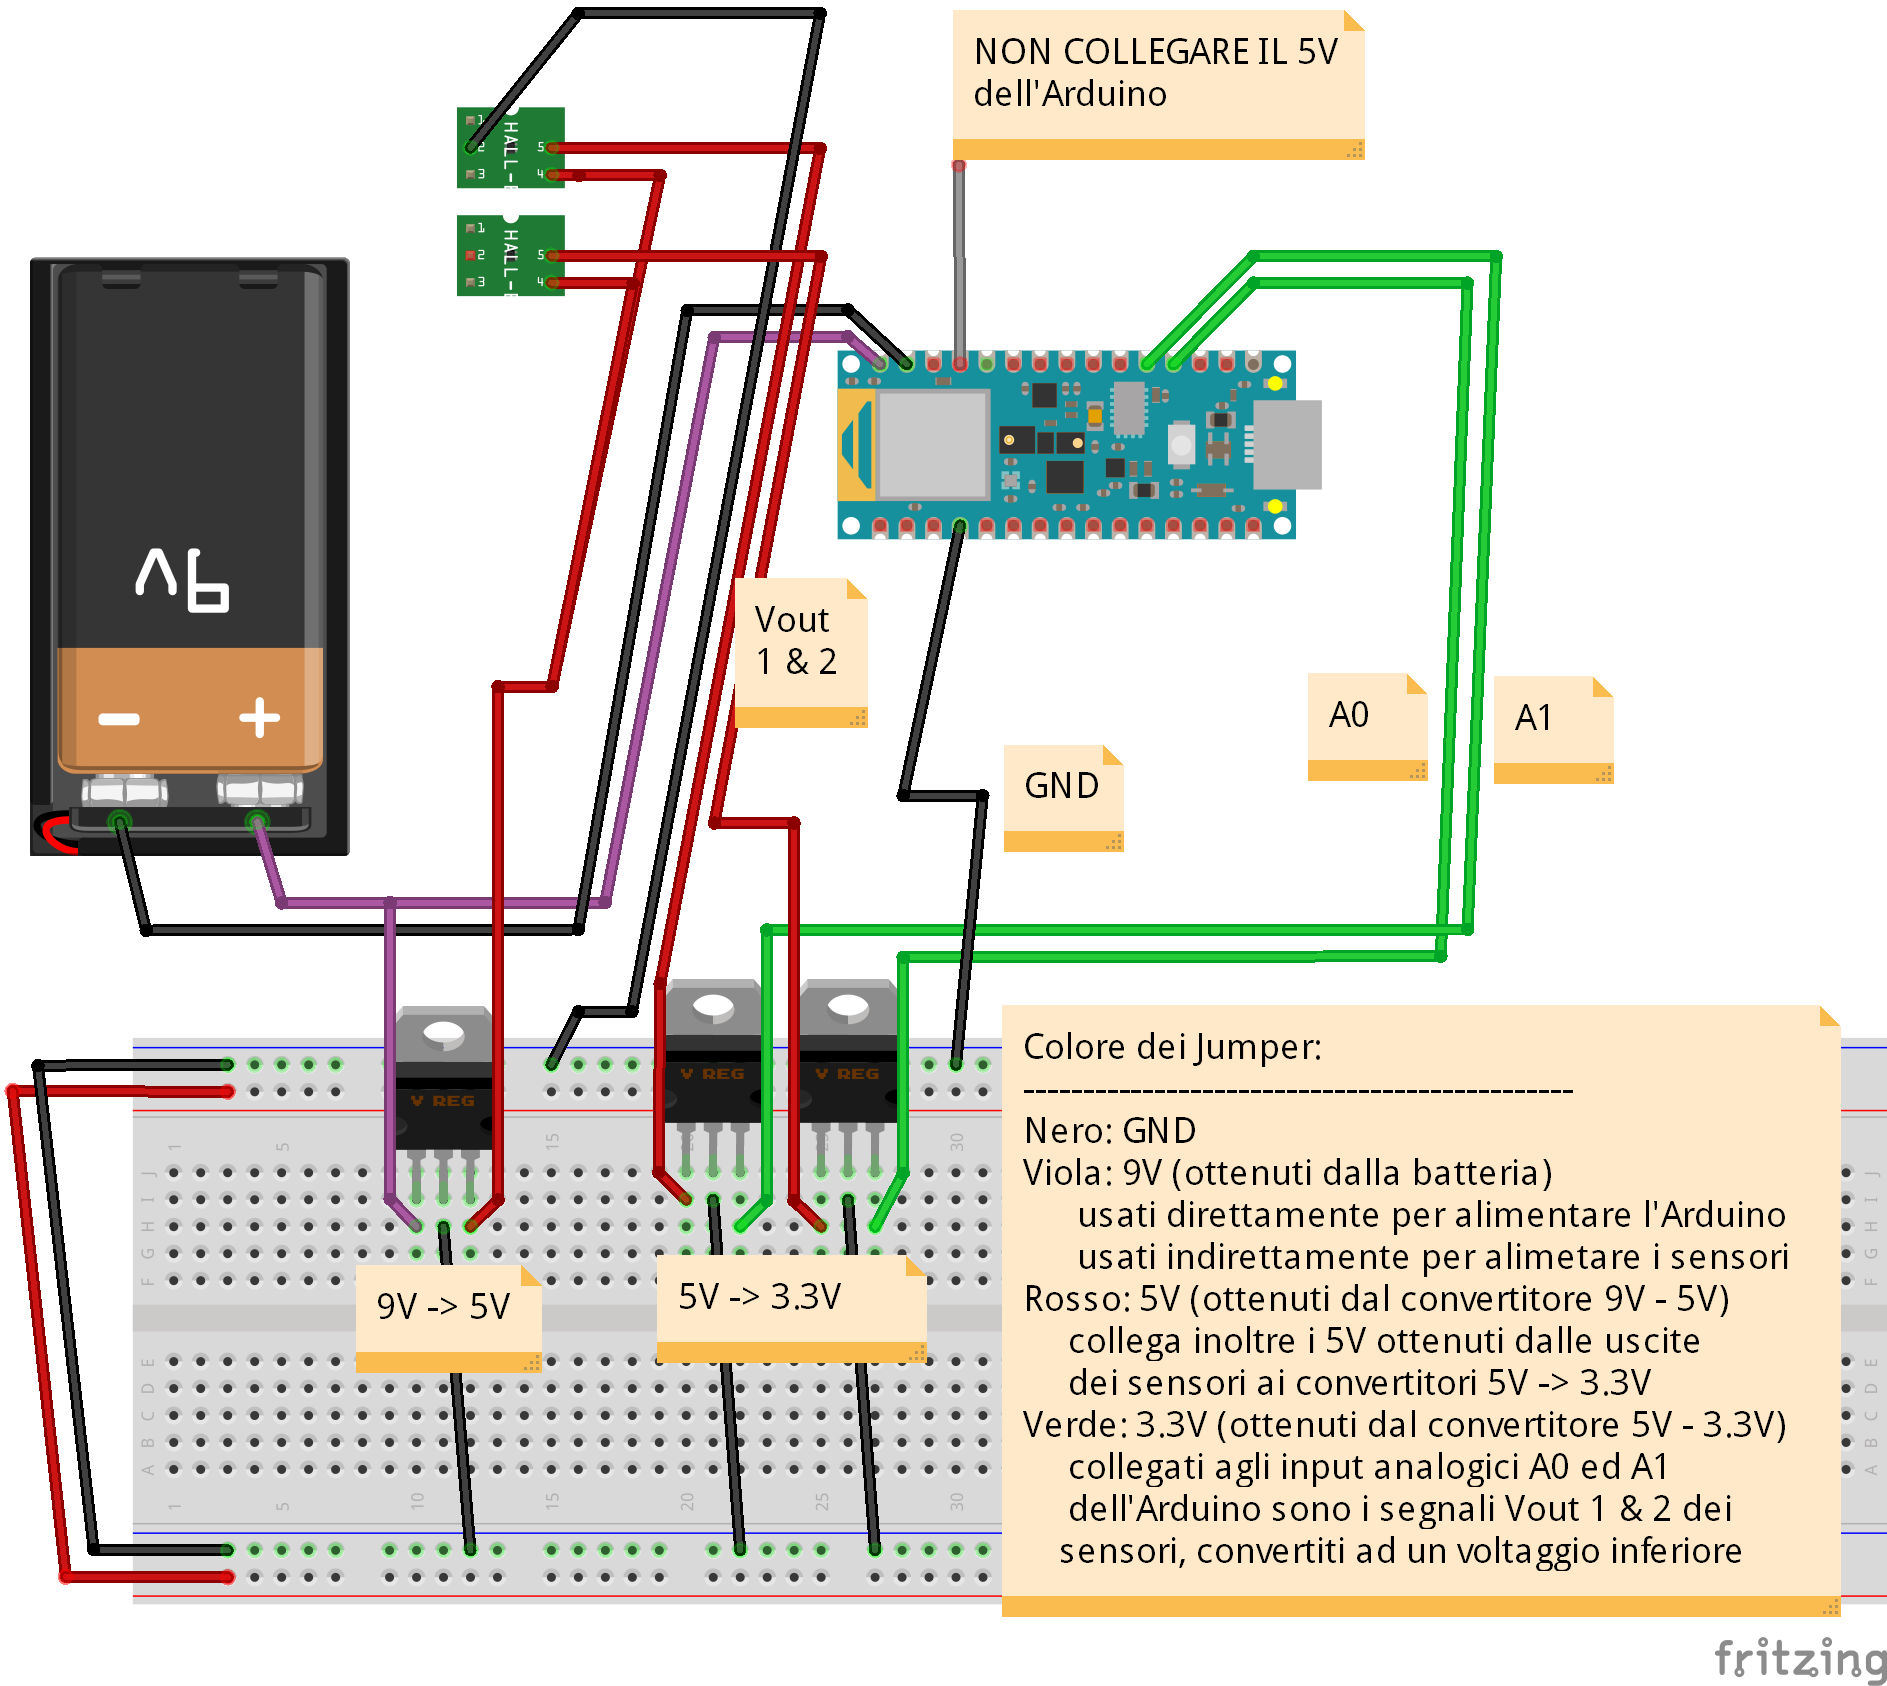
\includegraphics[width=\textwidth]{figures/2.1. Second Configuration -with more Names_bb.png}
    \caption{Esempio di hardware per la lettura dei sensori Hall su scheda Arduino Nano 33 BLE Sense}
\end{figure}

Tramite questa configurazione è possibile collegare l'Arduino Nano al PC per la raccolta dati tramite scrittura su seriale, utilizzando nel codice principalmente due funzioni: "AnalogRead(...)" e "Serial.print(...)", di seguito la parte principale del codice utilizzato per la lettura dai sensori:

\newpage{}

\begin{lstlisting}[language=Arduino]
void loop(){ // Lettura di due sensori
    String value_on_pollice = String(AnalogRead(A0));
    String value_on_medio = String(AnalogRead(A1));
    String timestamp = String(millis());
    Serial.println(timestamp + "," + value_on_pollice + "," + value_on_medio)
}
\end{lstlisting}






\subsection{Protocollo Edge Impulse} \label{sezione 2-1-1}
Il formato per la scrittura dei dati sul seriale:
\begin{lstlisting}[language=Arduino]
timestamp + "," + value_on_pollice + "," + value_on_medio
\end{lstlisting}
Non è stato scelto a caso, di fatti il servizio Edge Impulse richiede che i fogli ".csv" abbiano il seguente protocollo o formato, per la successiva lettura dei dati:
\begin{lstlisting}[language=HTML]
timestamp, name_value_1, name_value_2, name_value_3, name_value_4
0, 23.34, 2131.23, 321.23, 232.4
12, 23.34, 2131.23, 321.23, 232.4
23, 22.36, 2003.10, 321.23, 567.8
45, 26.24, 2056.40, 321.23, 567.9
54, 25.38, 1233.23, 321.23, 567.4
...
\end{lstlisting}
Questo formato sarà poi creato per intero dallo script python di cui parlerò nella prossima sezione, in ogni caso, è necessario che i fogli ".csv" abbiano tutti come prima colonna il "timestamp", così che Edge Impulse possa dare ad ogni dato fornitogli un marchio temporale, ecco il perché dell'omonima variabile durante la scrittura sul seriale (scritta appunto per prima).\\
Successivamente il sito si aspetta tutti i dati raccolti dai vari sensori, che vengono appunto scritti sul seriale, dopo il timestamp.

\subsection{Primo Prototipo del Guanto per la Raccolta Dati} \label{sezione 2-1-2}
A questo punto è necessario creare un prototipo per la raccolta dati, in quanto ho necessità di registrare i vari dati durante il movimento prestabilito, uno schiocco di dita.
Il prototipo con i sensori letteralmente incollati sopra è fondamentale per questo passaggio in quanto ho bisogno di avere i sensori nella stessa posizione, sia per l'allenamento, che per il test della rete neurale, se i sensori si muovessero ogni volta, addestrerei la rete su valori "traslati" rispetto alla fase di test, questo porterebbe sicuramente ad errori, non facilmente risolvibili.\par
Di seguito alcune foto su come ho incollato calamita e sensori, che poi collegherò alla scheda Nano come visto in precedenza in \riferimento{IMAGE - GDA ARDUINO NANO}{Figura 2.2}.

\label{IMAGE - GUANTO}
\begin{figure}[H]
    \centering
    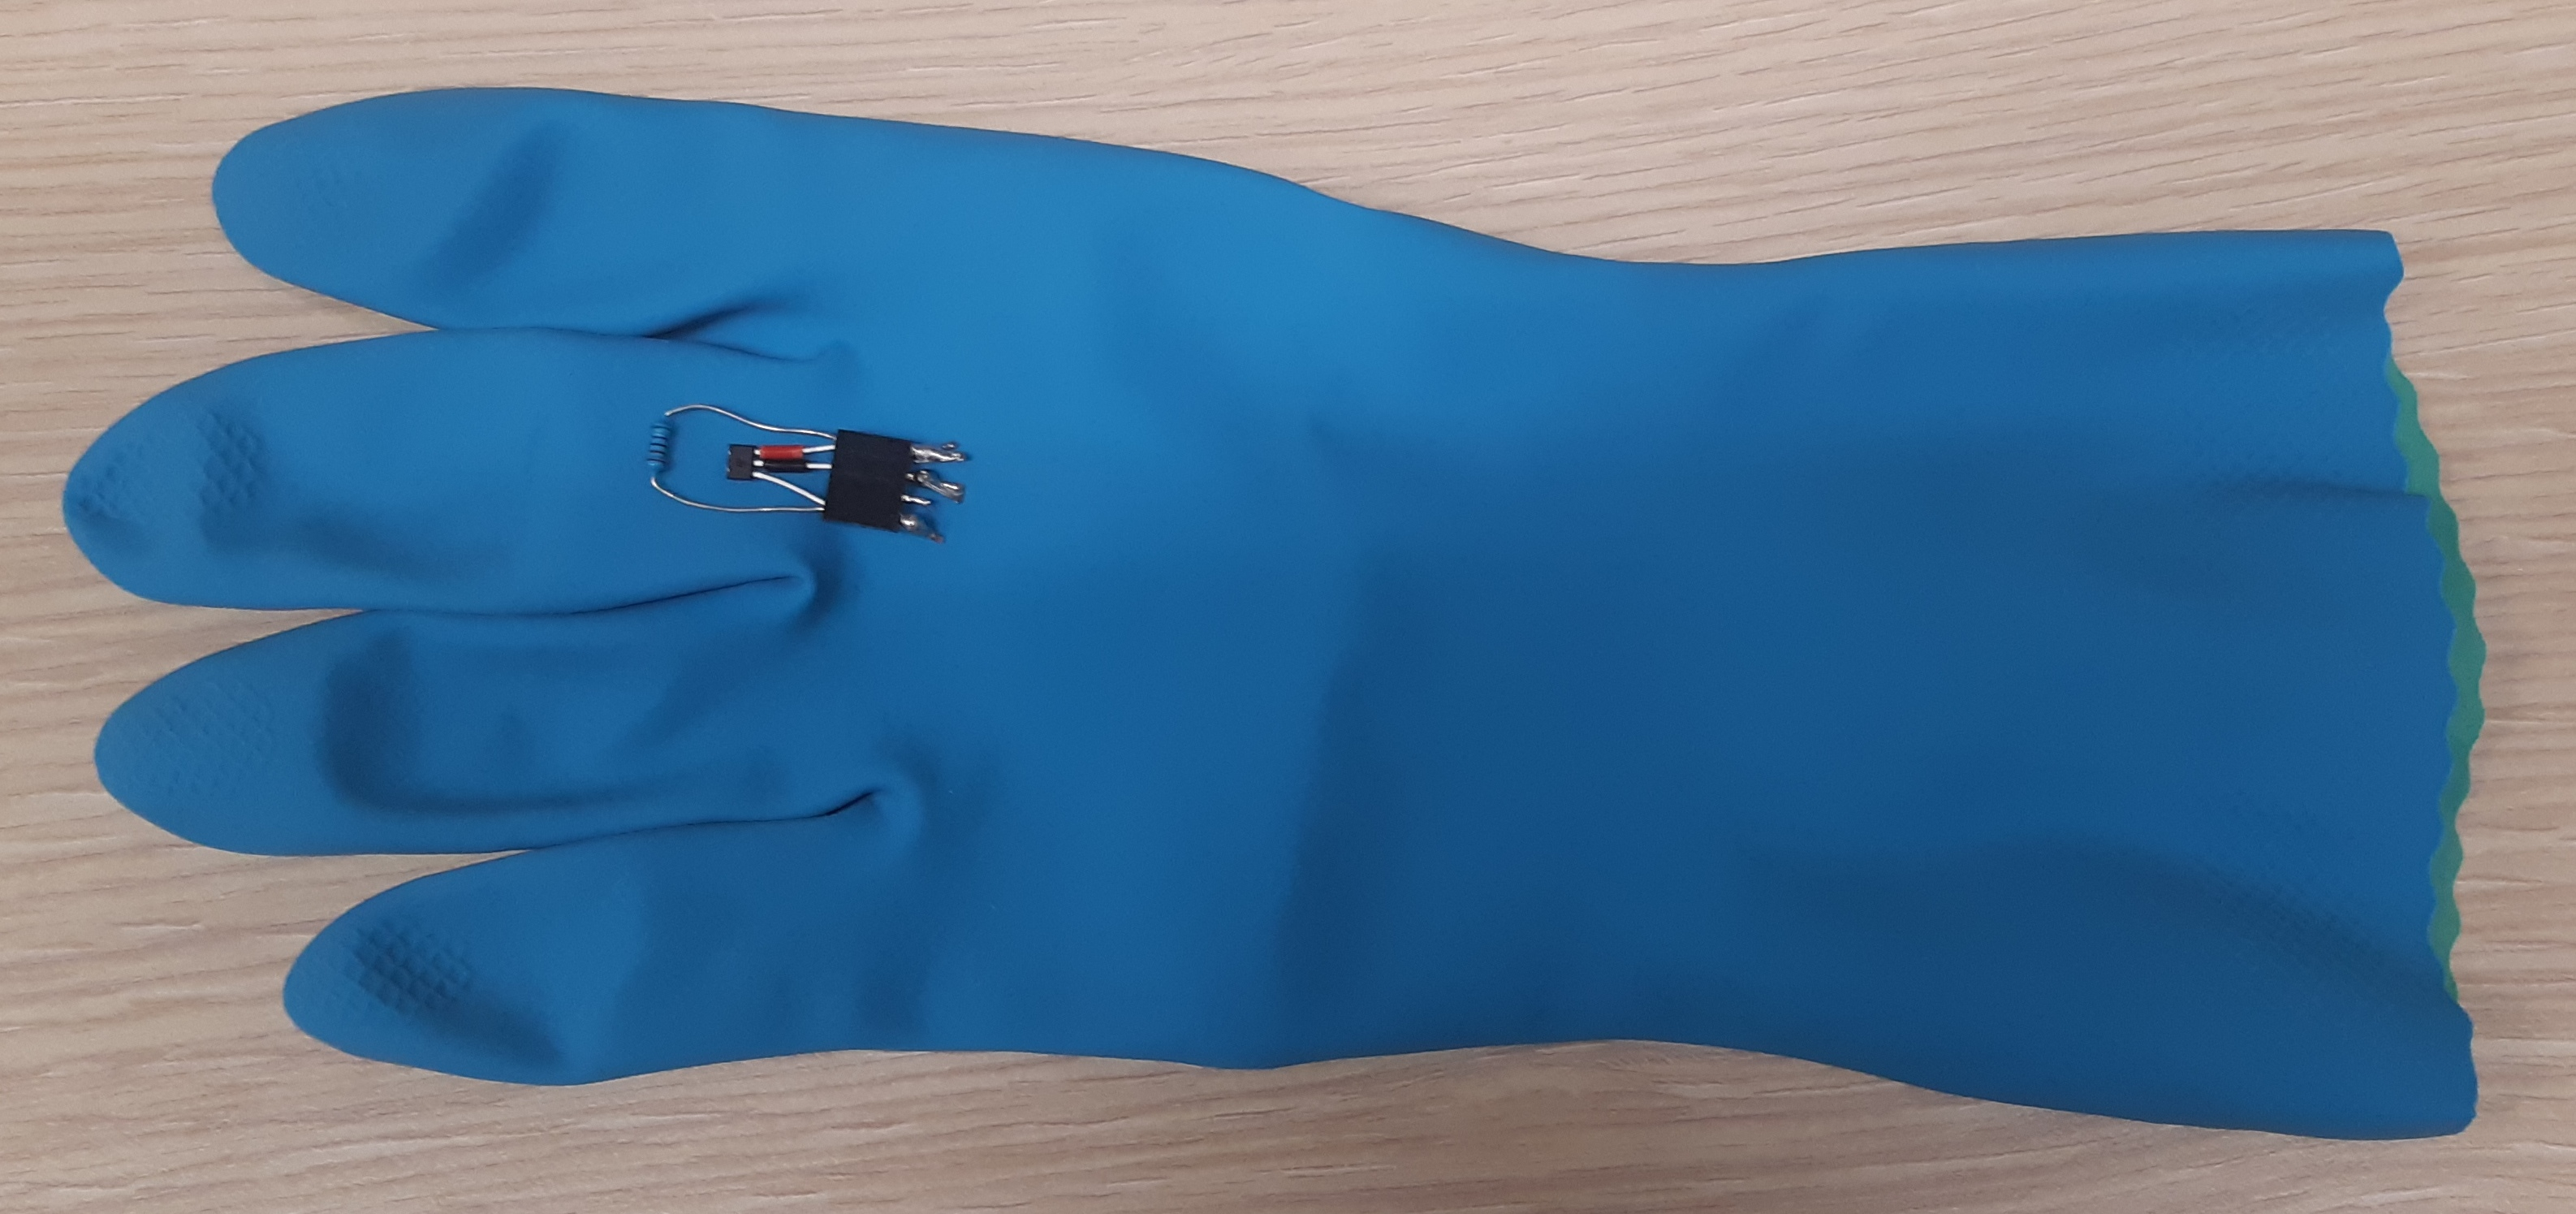
\includegraphics[width=115mm]{figures/Guanto_1 (1).jpg}
    \caption{Primo prototipo del guanto (sensore sul medio)}
    
    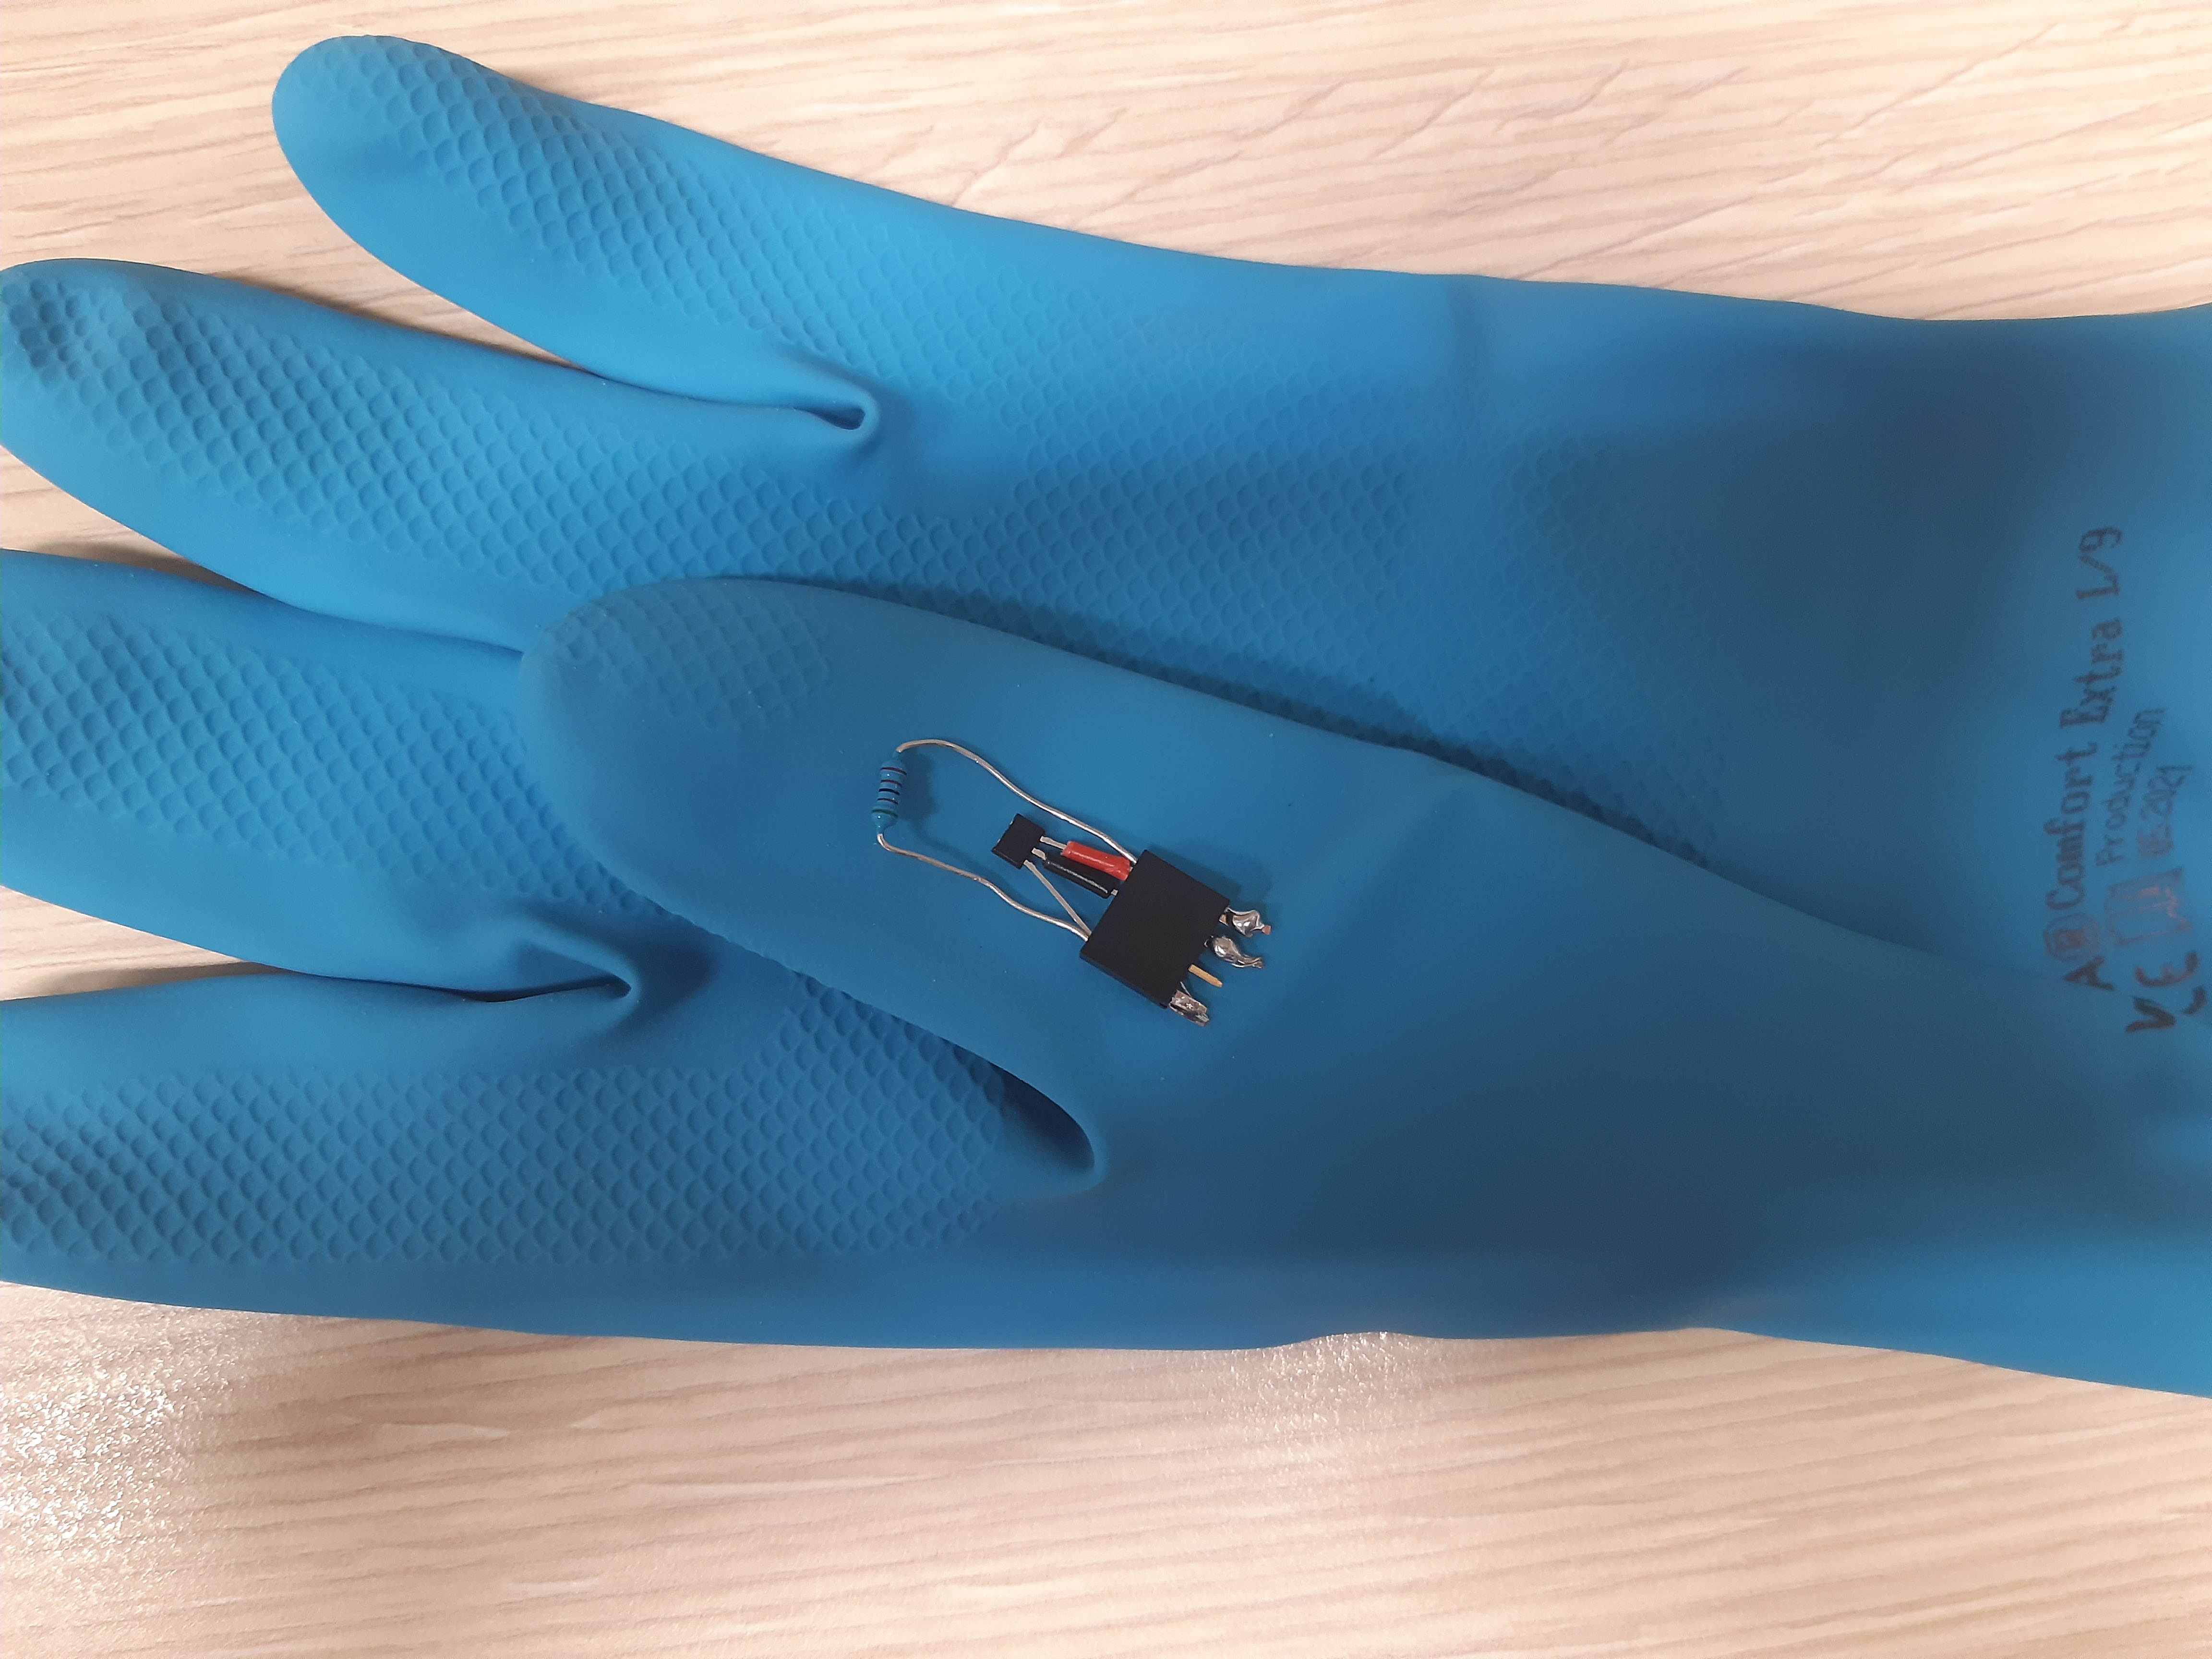
\includegraphics[width=115mm]{figures/Guanto_2.jpg}
    \caption{Sensore sul pollice}
    
    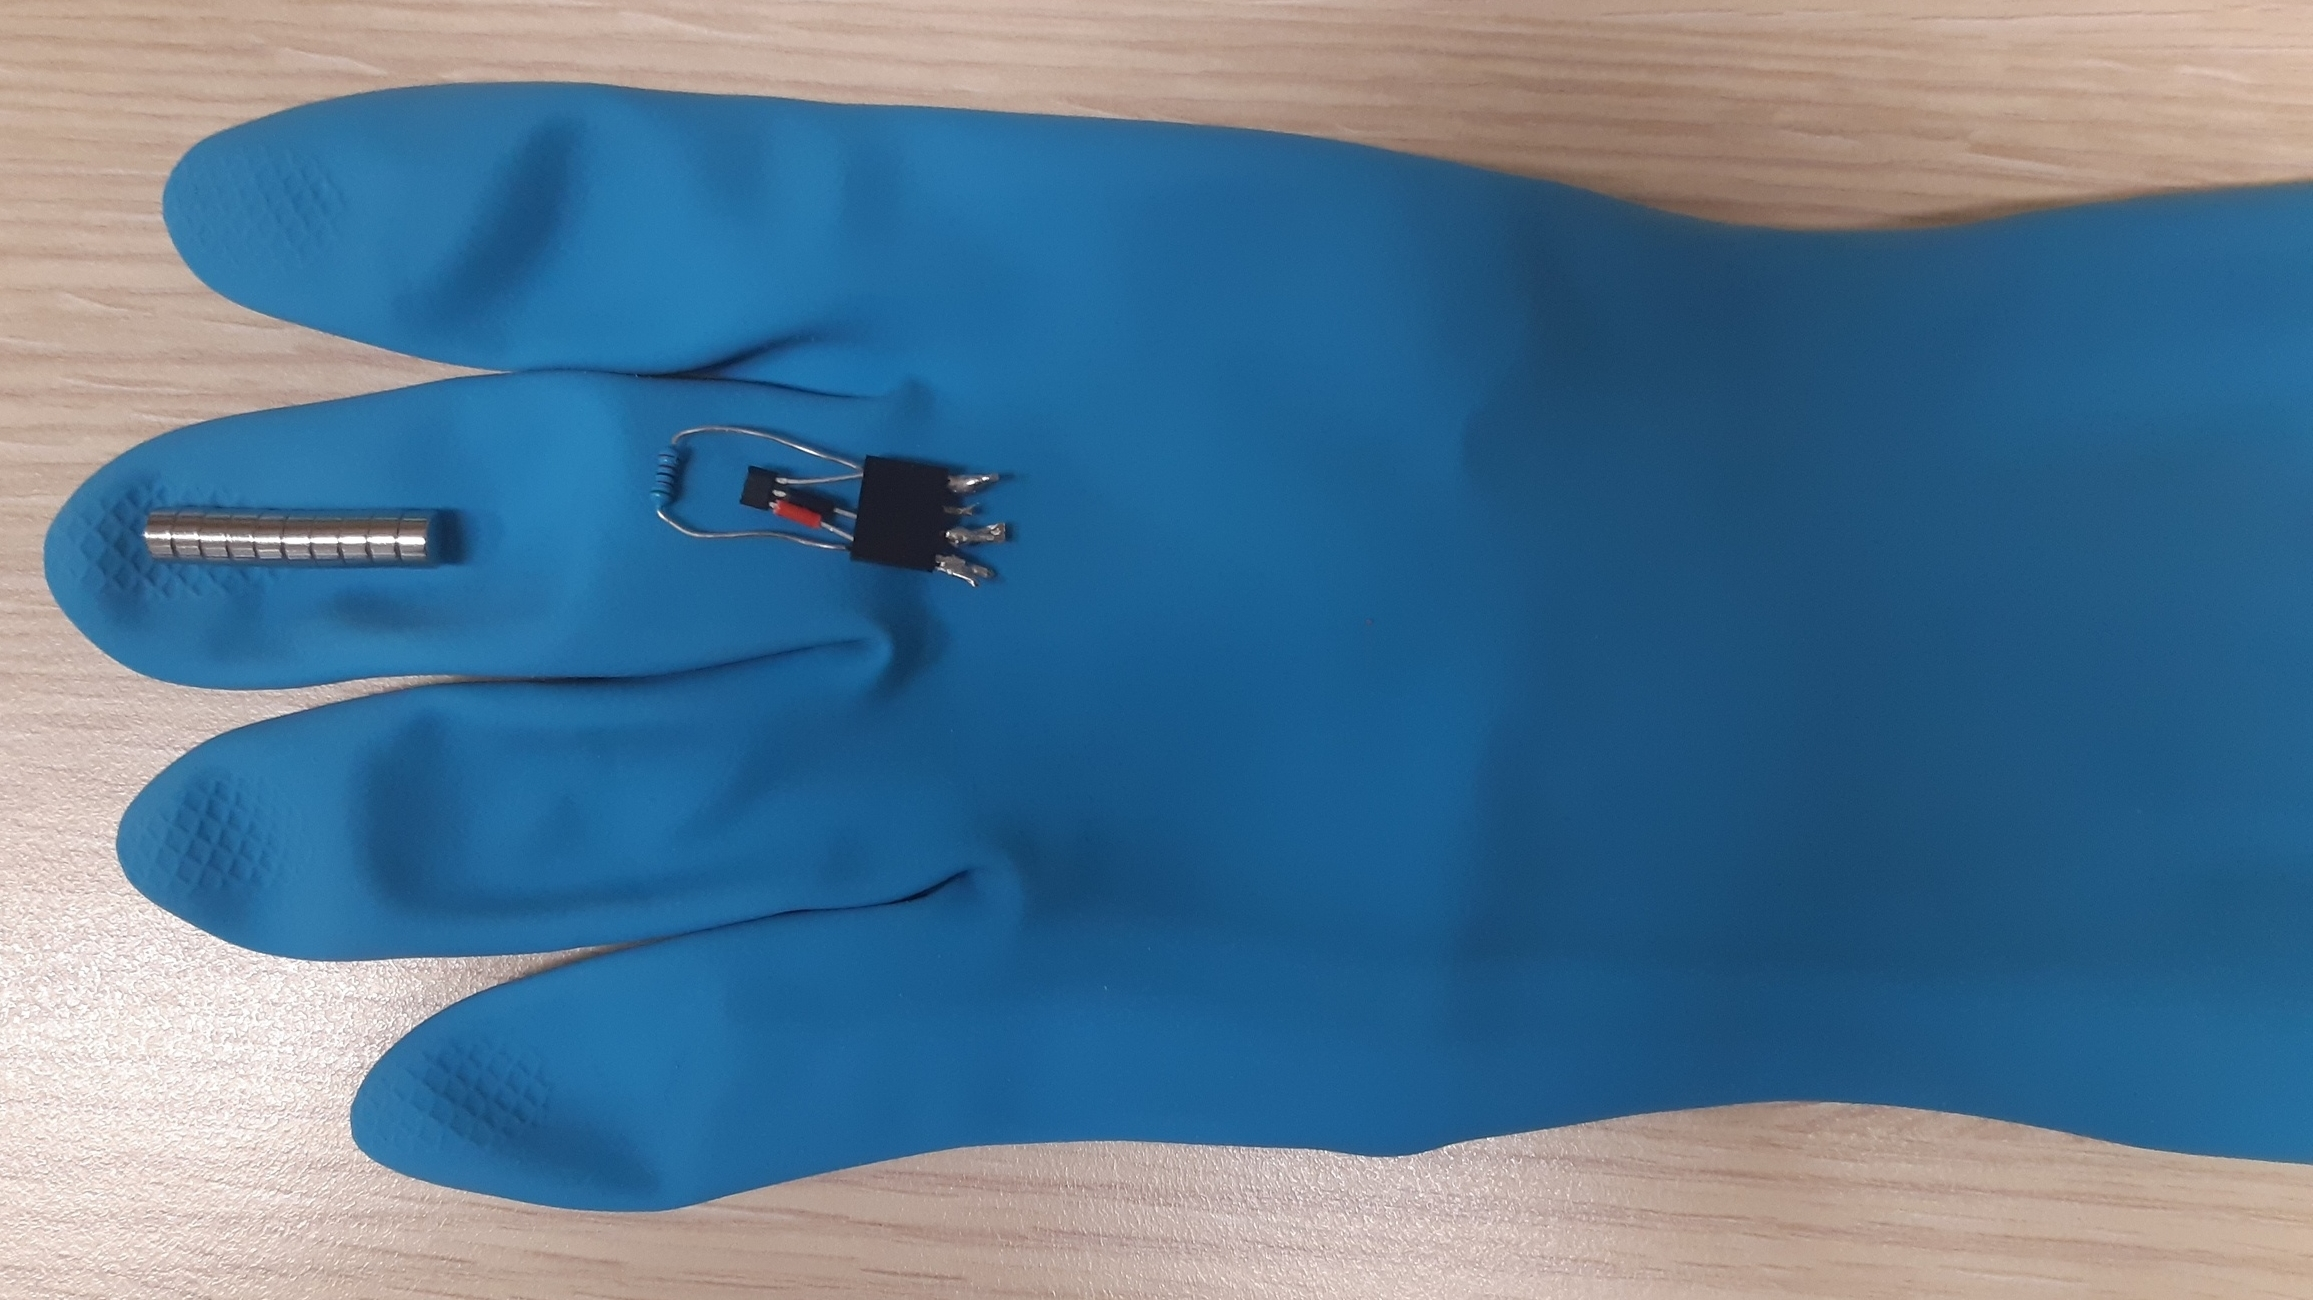
\includegraphics[width=115mm]{figures/guanto_3--3---1-.jpg}
    \caption{Sensore sul medio e calamita}
\end{figure}

\section{Script Python per la Scrittura Automatica di Fogli ".csv"} \label{sezione 2-2}
Ricevendo i dati tramite seriale è possibile utilizzare una libreria python "pyserial" per la lettura di questi; il procedimento è il seguente:
una volta collegata la scheda Arduino ad una porta seriale ad esempio "COM3", possiamo creare uno script python che utilizza la libreria o modulo "pyserial" in questo modo:
\begin{lstlisting}[language=Python]
import serial

MAX_CICLES = 100
EMPTY_DATA_SRING = "b''"
INITIAL_DATA_TO_INGNORE = len("b'")
FINAL_DATA_TO_INGNORE = len("'\n\r")

arduino = serial.Serial(
    port = 'COM3',
    baudrate = 115200, 
    timeout = .1
)

for _ in range(MAX_CICLES):
    data = str(arduino.readline())
    
    if data != EMPTY_DATA_SRING:
        return data[INITIAL_DATA_TO_INGNORE:-FINAL_DATA_TO_INGNORE]
\end{lstlisting}
\myNOTE{Questo breve script premette solo di leggere una singola riga dal serial. \\
Andrà ripetuto più volte per leggere tutti i dati passati dall'Arduino.}
\par{}Una volta ricevuti i dati dall'Arduino, e opzionalmente salvati in una variabile, sarà possibile scriverli su un nuovo foglio ".csv".\\
Decidendo il percorso dove salvare il file, ad esempio\\ "\textit{C:$\backslash{}$Users$\backslash{}$Amministratore$\backslash{}$Cartella\_Files\_CSV$\backslash{}$nuovo\_file.csv}", possiamo creare il file e trascriverci i dati da una variabile utilizzando la funzione python "open(...)":
\begin{lstlisting}[language=Python]
absolute_path = "C:\Users\Amministratore\Cartella_Files_CSV\nuovo_file.csv"
with open(absolute_path, "w") as file:
    file.write(dati_raccolti_dallArduino_tramite_la_precedente_funzione)
\end{lstlisting}

È possibile, ovviamente, ripetere tutto il procedimento quante volte vogliamo, finendo con\comment{pordandoci ad}  avere a disposizione molti fogli ".csv" con all'interno i dati ricavati dai sensori tramite la scheda Arduino, dati che saranno la base dell'addestramento della rete neurale.\\

Per la raccolta dati nel mio specifico caso ho fatto girare lo script python sia durante uno schiocco di dita, ma anche mentre tenevo\comment{ho tenuto} la mano ferma in varie posizioni diverse, ad esempio "mano aperta", "pugno chiuso" ecc., ed infine ho registrato anche alcune "anomalie", ovvero gesti che non devono essere classificati, questo per aiutare la rete neurale a distinguere in futuro tra uno schiocco di dita e tra un qualsiasi altro gesto, dopotutto lo scopo è far accendere dei led \textbf{solo} quando viene rivelato uno schiocco.
\newpage{}
\section{Utilizzo della Piattaforma Edge Impulse} \label{sezione 2-1}
Avendo a mia disposizione\comment{un totale di} più di 10 minuti di dati raccolti\comment{in questi file} nei file ".csv", ho creato ed addestrato la rete neurale utilizzando la piattaforma Edge Impulse:\\
Ho iniziato dopo la registrazione sul sito, creando un nuovo progetto, e caricando tutti i file creati in precedenza sull'apposita pagina, che si può trovare su 'Edge Impulse'$\rightarrow{}$'Data Aquisition'$\rightarrow{}$'Upload existing data', in questa pagina viene richiesto di caricare i file da inviare ad Edge, e scegliere un "label" che rappresenti tutti i file caricati, la label sarà poi utilizzata da Edge come classe di classificazione per la rete neurale.

Dopo viene chiesto di creare un cosiddetto "Impulso", ovvero il \textit{workflow} che implementerà Edge per l'addestramento del modello di machine learning. Per questo progetto la struttura dell'Impulso che ho scelto è la seguente:
\label{IMAGE - IMPULSO COMPLETO}
\begin{figure}[H]
    \centering
    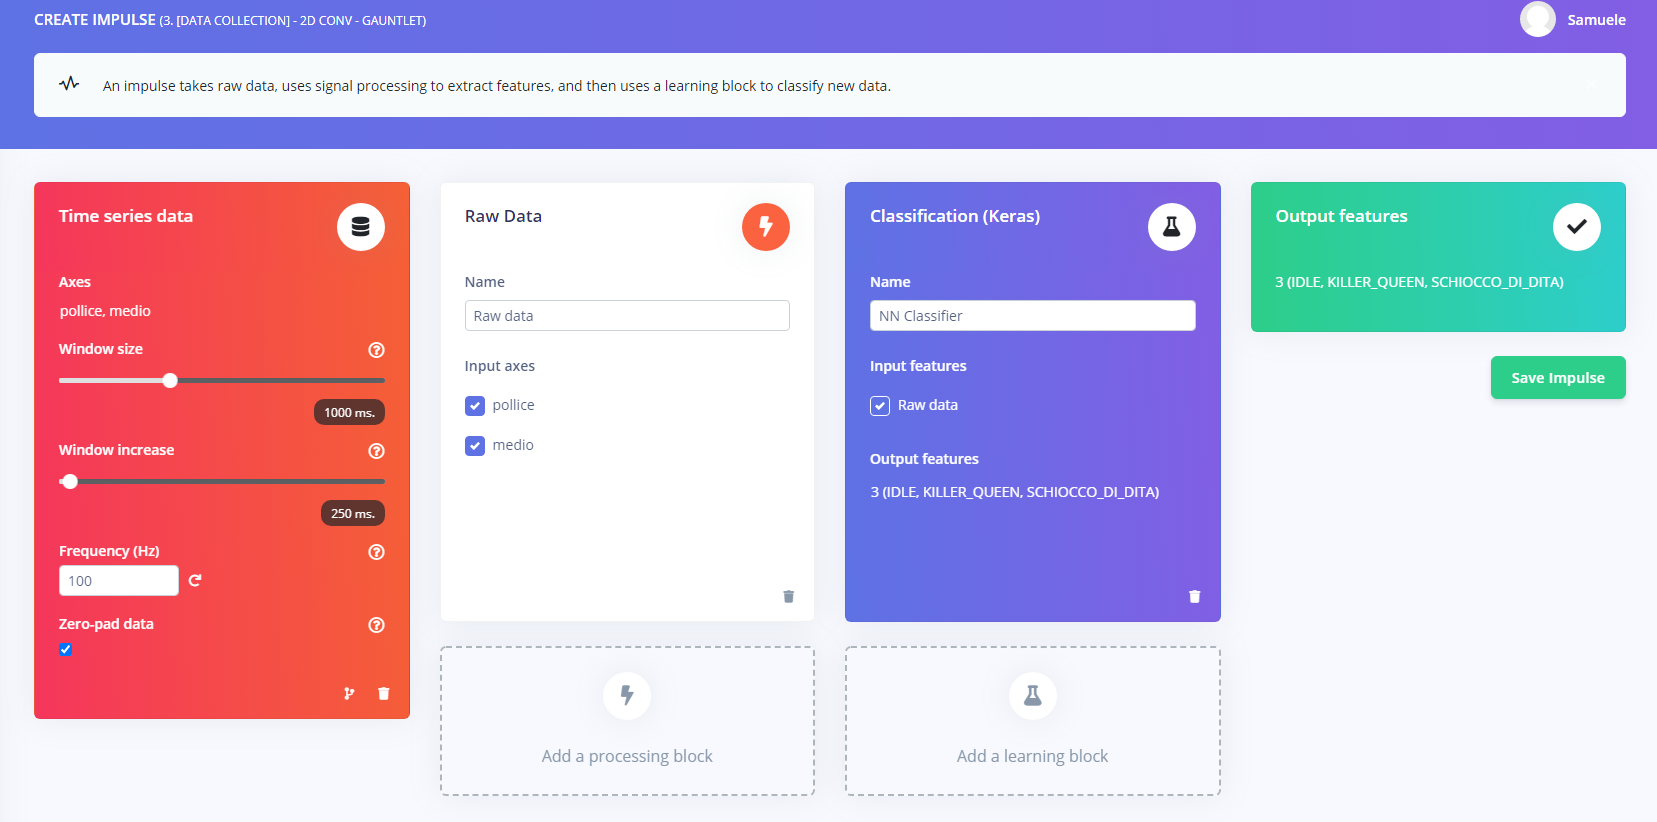
\includegraphics[width=\textwidth{}]{figures/Edge_Impulse_Impulso_Completo.PNG}
    \caption{Edge Impulse - Impulso Completo}
\end{figure}

\par{}'Time Series Data', indica principalmente la grandezza del vettore in ingresso al modello, rispetto al tempo (da qui la necessità del timestamp nel \riferimento{sezione 2-1-1}{Protocollo Edge Impulse}).
\par{}Il 'Blocco di Processo': 'Raw Data', indica che i dati ricevuti non dovranno essere modificati prima di essere passati alla rete neurale.
\par{}Mentre il 'Blocco di Apprendimento': 'Classification (Keras)', è una rete neurale costruita in python attraverso la libreria "keras" offerta da "TenserFlow".
\par{}Le 'Output Features', come accennato poco sopra sono i label digitati\comment{inseriti} durante l'upload dei file.\\

\newpage{}

\par{}A questo punto per completare l'Impulso è necessario specificare lo schema della rete neurale che dovrà essere utilizzata nel modello, dopo vari tentativi per testare quale potesse essere essere il miglior approccio, sono arrivato al seguente diagramma:
\label{IMAGE - NN CLASSIFIER}
\begin{figure}[H]
    \centering
    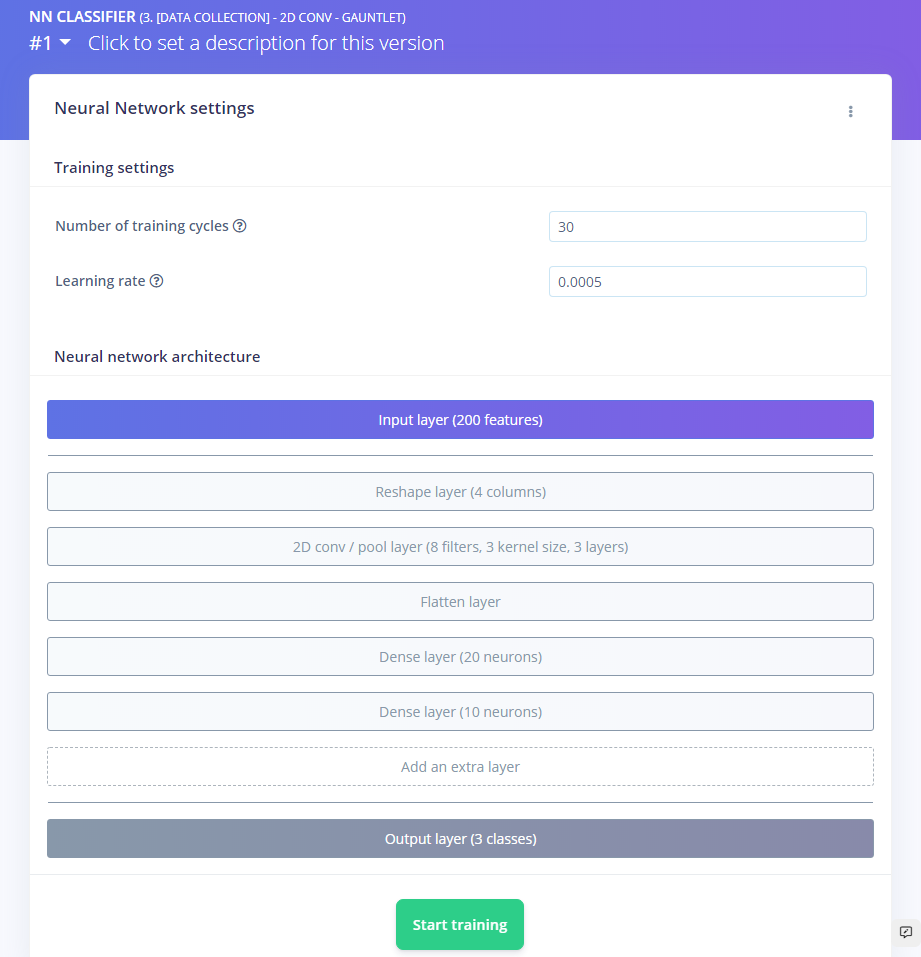
\includegraphics[width=\textwidth{}]{figures/Edge_Impulse_Gauntlet_NN_Classsifier.PNG}
    \caption{Edge Impulse - Rete Neurale}
\end{figure}

\newpage{}

Cliccando su "Start training", dopo pochi minuti, ci viene fornita oltre all'accuratezza rispetto al set di '\textit{cross-validation}', anche una stima delle prestazioni che avrà il modello una volta dislocato sulla piattaforma embedded scelta, ed una utile \textit{confusion matrix}, che indica per quale/i classi il modello ha una peggiore capacità di classificazione.
\label{IMAGE - TRAINING}
\begin{figure}[H]
    \centering
    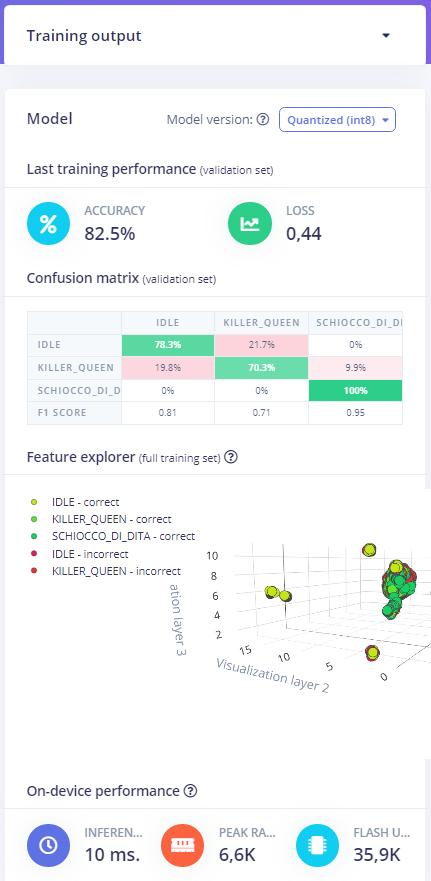
\includegraphics[width=90mm]{figures/Edge_Impulse_Training.PNG}
    \caption{Edge Impulse - Risultati Addestramento}
\end{figure}

La rete neurale è conclusa, rimane solo da portarla sulla scheda Arduino sotto forma di modello di TensorFlow Lite.\\
Rechiamoci quindi, alla parte di "\textit{Deployment}" di Edge Impulse e scegliamo l'opzione \\"\textit{Arduino Library}":
\label{IMAGE - DEPLOYMENT}
\begin{figure}[H]
    \centering
    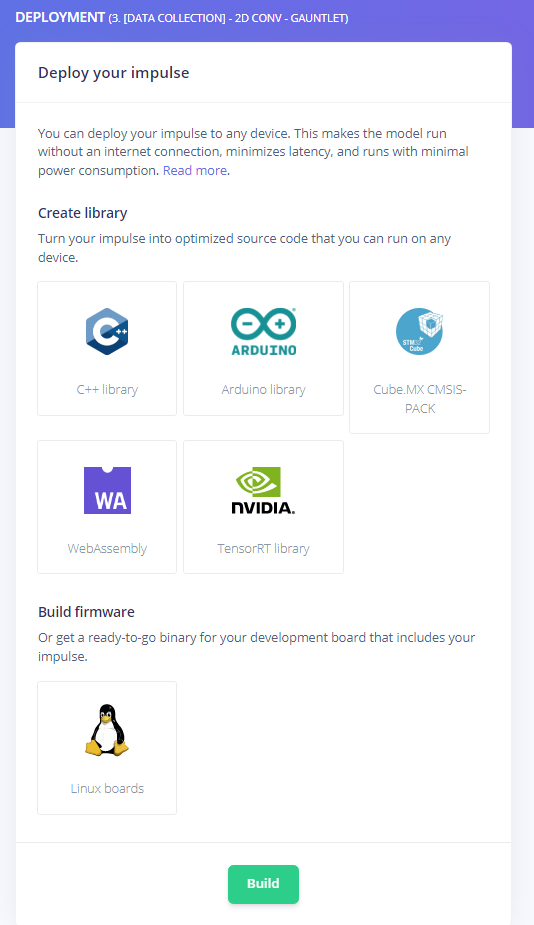
\includegraphics[width=100mm]{figures/Edge_Impulse_Deployment.PNG}
    \caption{Edge Impulse - Deployment}
\end{figure}
Ci verrà fornita una libreria ".zip" che potrà essere aggiunta dall'Arduino IDE da:\\ Sketch$\rightarrow{}$\#include libreria$\rightarrow{}$Aggiungi libreria da file .ZIP...




\section{Utilizzo della Libreria Offerta da Edge Impulse} \label{sezione 2-4}
Una volta scaricata la libreria da "Edge Impulse", la possiamo includere su un nuovo sketch Arduino, e caricare un codice esempio\comment{compreso nella} dalla stessa libreria, dal nome "static\_buffer":
\label{IMAGE - DEPLOYMENT}
\begin{figure}[H]
    \centering
    \caption{Arduino IDE - static\_buffer example}
    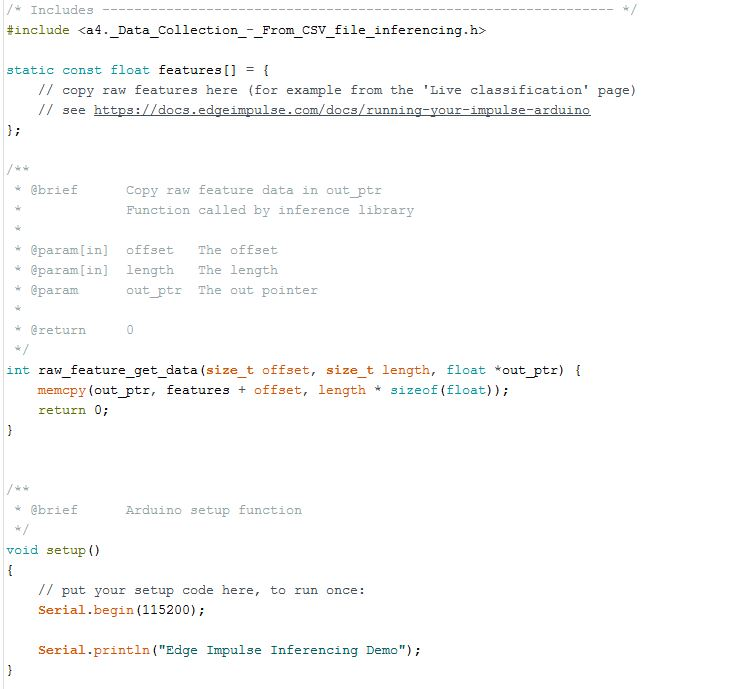
\includegraphics[width=\textwidth{}]{figures/Edge_static_buffer_Setup.JPG}
\end{figure}

\newpage{}

In questo esempio ci è consigliato di modificare, o meglio, riempire il vettore "features[ ]" con i dati presi dai sensori, quindi utilizzando lo stesso metodo per la raccolta dati, riempiamo il vettore:
\begin{lstlisting}[language=Arduino]
void loop(){
    int length_featrues = sizeof(features)/sizeof(float);
    for(int i = 1; i < length_features; i++){
        features[i-1] = features[i];
    }
    features[length_featrues-1] = new_data_just_aquired
}
\end{lstlisting}
Dopodiché nell'esempio il vettore viene passato in una serie di funzioni per poter poi essere usato dal classificatore, o rete neurale:
\begin{lstlisting}[language=Arduino]
    int raw_feature_get_data(size_t offset, size_t length, float *out_ptr) {
        memcpy(out_ptr, features + offset, length * sizeof(float));
        return 0;
    }

    // the features are stored into flash, and we don't want 
    // to load everything into RAM
    signal_t features_signal;
    features_signal.total_length = sizeof(features) / sizeof(features[0]);
    features_signal.get_data = &raw_feature_get_data;

    // invoke the impulse
    EI_IMPULSE_ERROR res = run_classifier(
    &features_signal, &result, false /* debug */);
    
    // -----------------------------------------------------------------------
    // TEMPI DEL CLASSIFICATORE
    // result.timing.dsp
    // result.timing.classification
    // result.timing.anomaly
    
    // DETTAGLI:
    // result.classification[ix].label
    // result.classification[ix].value
    // result.anomaly
\end{lstlisting}

Quindi con \lstinline{result.classification[ix].label}, \lstinline{result.classification[ix].value}, e \lstinline{result.anomaly} è possibile implementare il resto del codice:

\begin{lstlisting}[language=Arduino]
    if(result.classification[ix].label == "SCHIOCCO_DI_DITA"){
        if(result.classification[ix].value > 0.9){
            // Light the leds
            digitalWrite(A2, HIGH);
            
            // Empty features[] vector
            float new_blank_float[lenght_features];
            features = new_blank_float;
            
            delay(2000);
            
            // Kill the ligths
            digitalWrite(A2, LOW);
        }
    }
\end{lstlisting}

\myNOTE{
In questo caso \lstinline{result.anomaly} non è stata implementata. In caso si volesse implementare\\
è possibile, tornando alla costruzione dell'Impulso nella sezione precedente, aggiungendo\\
un nuovo "Blocco di Apprendimento" chiamato "Anomaly Detection (K-means)" che\\ 
tramite un algoritmo di K-clustering ritorna un valore, sempre tra 0 ed 1, indicativo di\\ 
quanto è probabile che la classificazione trovata sia un anomalia, in caso questo se il valore\\
fosse elevato, la classificazione va considerata errata e deve essere scartata.
}
\clearpage\null\thispagestyle{empty}

\addcontentsline{toc}{chapter}{Conclusioni}
\chapter*{Conclusioni}


\label{98-Conclusioni}
Il progetto, una volta finito, è in grado di rivelare la maggior parte degli schiocchi effettuati (71\%): problemi sorgono tuttavia quando non si effettua uno schiocco, infatti muovendo leggermente la mano viene effettuata talvolta una lettura sbagliata, soprattutto quando viene mosso il pollice (sul quale è presente un sensore). In questo caso, il movimento non viene classificato come un anomalia ma come uno schiocco, causando l'accensione dei led.
Alcune fra le possibili cause alla base di questa problematica potrebbero essere:\\

\noindent{}Il modello utilizzato è in una condizione di "overfitting", ovvero il modello si è abituato ai dati dati nel training set, e classifica in modo errato i dati effettivi; un segnale d'allarme per questo particolare caso è dato dal "Model Testing" su Edge Impulse che riporta un'accuratezza \textbf{teorica} del modello pari al 80\%.\\

\noindent{}I dati sulle anomalie sono insufficienti. Semplicemente raccogliendo più dati, sopratutto su molti casi nei quali l'utente \textbf{non} schiocca le dita, è possibile allenare il modello a distinguere le due classi in maniera più accurata.\\

\noindent{}I sensori utilizzati non sono ottimali per il lavoro da eseguire; i sensori di Hall riportano una grande variazione ad un piccolo movimento se il sensore è molto vicino alla calamita (< 5 cm). Diversamente, ad una distanza maggiore di 5 cm il sensore rivelerà una piccolissima variazione di tensione in caso di movimento del magnete (al minimo 1.3 mV), mentre ad una distanza superiore ai 7.5 cm non verrà rilevata nessuna variazione di tensione.\\

\noindent{}Infine, i dati non stati modificati in alcun modo prima di essere passati alla rete neurale, quindi creando un nuovo "Processing Block" su Edge Impulse, oppure modificando direttamente i dati inviati dall'Arduino, è possibile facilitare l'addestramento della rete neurale.\\

\addcontentsline{toc}{chapter}{Bibliografia}
\chapter*{Bibliografia}


\newcommand{\bibNum}[1]{\noindent{}\textbf{\lbrack{}}#1\textbf{\rbrack{}}}


\label{100-chapter}

\bibNum{1}  "Edge Impulse - pagina iniziale", https://www.edgeimpulse.com/. URL

\bibNum{2} "TensorFlow - pagina iniziale", https://www.tensorflow.org/lite. URL

\bibNum{3} "Arduino Nano 33 BLE Sense", Arduino Shop,\\ \indent{}https://store.arduino.cc/products/arduino-nano-33-ble-sense?selectedStore=eu. URL

\bibNum{4} "Arduino IDE Download", Arduino, https://www.arduino.cc/en/software. URL

\bibNum{5} S. Petrizzelli, “Appunti di fisica 2- effetto hall".\\
\indent{}http://users.libero.it/sandry/Fisica2-002.pdf. URL\

\bibNum{6} "Effetto Hall", Wikipedia L'enciclopedia libera, \\
\indent{}https://it.wikipedia.org/wiki/Effetto\_Hall. URL

\bibNum{7} Allegro Microsystems Inc. A1301 Datasheet, \\
\indent{}A1https://docs.rs-online.com/872c/0900766b80d88057.pdf. URL

\bibNum{8} "Edge impulse: un intuitivo SDK", Elettronica Open Source\\ \indent{}https://it.emcelettronica.com/edge-impulse-un-intuitivo-sdk-per-il-tinyml-parte-i. URL


\addcontentsline{toc}{chapter}{Ringraziamenti}
\chapter*{Ringraziamenti}

\label{101-chapter}
Vorrei ringraziare tutte le persone che mi hanno aiutato a svolgere il progetto, e compilare questa tesi:\\
\par{}\textbf{\textit{Alessandro Pozzebon}}.\\
\par{}\textbf{\textit{Stefano Parrino}}.\\
\par{}\textbf{\textit{Stefano Frigerio}}.\\
\par{}\textbf{\textit{Garbiele Di Renzone}}.\\
\par{}\textbf{\textit{Giacomo Peruzzi}}.\\


%\chapter{TODO NAME OF CODE CHAPTER}
%

\label{capitolo99}

\section{Introduzione al capitolo} \label{99-1}
TODO INTRODUZIONE

\section{TODO NOME SEZIONE 99-1} \label{99-1}



\subsection{Funzione: nome\_funzione(...)}
\noindent{piccola descrizione}
\begin{lstlisting}[language=Arduino]
//SCRIVI QUI IL CODICE
\end{lstlisting}
\noindent\makebox[\linewidth]{\rule{15mm}{.4mm}}


\subsection{Funzione: nome\_funzione(...)}
\noindent{piccola descrizione}
\begin{lstlisting}[language=Arduino]
//SCRIVI QUI IL CODICE
\end{lstlisting}
\noindent\makebox[\linewidth]{\rule{15mm}{.4mm}}


\subsection{Funzione: nome\_funzione(...)}
\noindent{piccola descrizione}
\begin{lstlisting}[language=Arduino]
//SCRIVI QUI IL CODICE
\end{lstlisting}
\noindent\makebox[\linewidth]{\rule{15mm}{.4mm}}


\subsection{Funzione: nome\_funzione(...)}
\noindent{piccola descrizione}
\begin{lstlisting}[language=Arduino]
//SCRIVI QUI IL CODICE
\end{lstlisting}
\noindent\makebox[\linewidth]{\rule{15mm}{.4mm}}


\subsection{Funzione: nome\_funzione(...)}
\noindent{piccola descrizione}
\begin{lstlisting}[language=Arduino]
//SCRIVI QUI IL CODICE
\end{lstlisting}
\noindent\makebox[\linewidth]{\rule{15mm}{.4mm}}


\subsection{Funzione: nome\_funzione(...)}
\noindent{piccola descrizione}
\begin{lstlisting}[language=Arduino]
//SCRIVI QUI IL CODICE
\end{lstlisting}
\noindent\makebox[\linewidth]{\rule{15mm}{.4mm}}


\subsection{Funzione: nome\_funzione(...)}
\noindent{piccola descrizione}
\begin{lstlisting}[language=Arduino]
//SCRIVI QUI IL CODICE
\end{lstlisting}
\noindent\makebox[\linewidth]{\rule{15mm}{.4mm}}

\end{document}
